\documentclass[nofilelist]{cslthse-msc}
% to show a list of used packages at the end of the document, delete the nofilelist option
%\documentclass{cslthse-msc} 
\usepackage[utf8]{inputenc}
\usepackage[english]{babel}
\usepackage{amsmath}
%\usepackage{amsfonts}
%%\usepackage{amssymb}
\usepackage{amsthm}
%\usepackage{makeidx}
\usepackage{graphicx}
\usepackage[titletoc, header, page]{appendix}
\usepackage{transparent}
\usepackage{algpseudocode}
\usepackage{amsmath}
\usepackage{titlesec}

% used to display the used files at the end. Select nofilelist as a package option to disable this
\listfiles % initialize

%\geometry{showframe}
%better like this?
\student{Alexander Sandström}{alexander.h.sandstrom@gmail.com}
%\students{Flavius Gruian}{Flavius.Gruian@cs.lth.se}{Camilla Lekebjer}{Camilla.Lekebjer@cs.lth.se}

\thesisnumber{} % Magic Number! Do not change unless Birger Swahn asks you to do so!
% default is Master. Uncomment the following for "kandidatarbete"/Bachelor's thesis
%\thesistype{Bachelor}{Kandidatarbete}

%\title{Formatting a Master's Thesis}
\title{Drones for Sea Rescue: Lab and Field Experiments on Camera Gimbal Control}
\svensktitel{Drönare inom Sjöräddning: en Studie i Operatörsupplevelse av Kamerakontroll}


%\onelinetitle
%\twolinestitle
\threelinestitle
%\fourlinestitle

%\subtitle{A suitable subtitle}
\company{the Swedish Sea Rescue Society and the Department of Electrical and Information Technology, Lund University}
\supervisors{Fredrik Falkman, \href{mailto:fredrik.falkman@ssrs.se}{\texttt{fredrik.falkman@ssrs.se}}}{William Tärneberg, \href{mailto:william.tarneberg@eit.lth.se}{\texttt{william.tarneberg@eit.lth.se}}}
\examiner{Maria Kihl, \href{mailto:maria.kihl@eit.lth.se}{\texttt{maria.kihl@eit.lth.se}}}

\date{\today}
%\date{January 16, 2015}

\acknowledgements{
If you want to thank people, do it here, on a separate right-hand page. Both the U.S. \textit{acknowledgments} and the British \textit{acknowledgements} spellings are acceptable.

}

\theabstract{
The Swedish Sea Rescue Society (SSRS), responsible for 90\% of sea rescue in Sweden, are running a project with Chalmers, Infotiv, Airpelago and RISE called Eyes-on-Scene (EOS), investigating the use of drones to provide early imagery of a maritime incident to rescue personnell on their way to the scene. 

Thus far in the project, a fixed-wing drone along with mission control software has been developed, and the drone is able to fly after waypoints while providing video through the gimbal-mounted camera. The drone has a 4G modem, allowing it to be operated beyond visual line-of-sight (BVLOS). 

With the current software, the SSRS do not have a way to manually control the direction of the camera, and wanted direct control with either a joystick or the arrow keys. The SSRS was also interested in investigating if the manual controls were suitable with the delay introduced by the mobile connection.

In this thesis work, a gimbal control interface has been developed with the aim of acheiving manual control of the camera while also studying the effects of latency on the operator's experience. Two experiments have been carried out: one user study, evaluating quantative and qualitative effects of latency on a camera operator, and one field test, where the gimbal control software was tested during a flight over the Gothenburg archipelago.

In the user study, the user was given a task to perform provided a joystick and a video feed from the drone camera. Five trials with simulated latencies were performed per subject. The results of the study indicate that the relationship between latency and task performance might not be linear, and that an equal amount of delay increase can have different effects on operator experience at different levels of latency.

In the second experiment, the field test, the software was successfully integrated with the in-flight systems and a test flight was made over the Gothenburg Archipelago. The manual controls using a joystick were deemed suitable, although delay and rapid movements of the drone could introduce difficulty.  
}

\keywords{MSc, BSc, template, report, style, structure}

%% Only used to display font sizes
\makeatletter
\newcommand\thefontsize[1]{{#1 \f@size pt\par}}
\makeatother
%%%%%%%%%%

\begin{document}
\renewcommand{\bibname}{References}

\makefrontmatter
\chapter{Introduction}
The use of UAVs have skyrocketed during the last decade, and due to advancements in technology as well as legislature, a once mainly military technology is now seeing more use in the civilian sector with uses in cinematography, agriculture as well as search and rescue. The main selling point of the UAV is its' ability to provide aerial data (usually imagery) at a fraction of the cost of manned aircraft, making it a viable alternative for many expensive, remote or even dangerous applications.

The use of drones and other small electric vehicles in research as well as in the DIY-space has led to the rise of several open-source software initiatives which provide both the software running on the vehicle as well as the ground control software (GCS) used for planning and monitoring missions. 

Although rotor drones are the most common consumer drones, fixed-wing drones have seen a rise in use, mainly for their increased battery time and speed. In spite of these advantages, obtaining imagery from a fixed-wing drone remains more difficult than from a rotor drone as the fixed-wing needs airspeed to stay in flight and will thus eventually fly past a stationary target. In order to solve this problem, a mechanical gimbal can be used to change the direction of the camera. The operator can also be assisted by software which can adjust the direction of the camera based on the drone's position and orientation, either just to stabilize the video feed in some of the axes or to target a stationary GPS-point.

The Swedish Sea Rescue Society (SSRS) are running a project with Chalmers, Infotiv, Airpelago and RISE called Eyes-on-Scene (EOS), investigating the use of drones to provide early imagery of a maritime incident to rescue personnell on their way to the scene. In the project a fixed-wing drone carrying a gimbal-mounted camera has been developed on the open-source platform ArduPilot. A web application has been built to easen the process of planning and monitoring missions as well as providing and recording the video feed from the drone camera.

In the project thus far, the drone has flown several waypoint missions in the archipelago of Gothenburg where the SSRS has a permit to operate drones BVLOS. A problem for the SSRS has been to control the direction of the camera, as the only way to do so has been to upload a GPS-point to the drone towards which the autopilot will point the camera. This is a cumbersome process due to the many steps involved in uploading an ROI. An ROI is also susceptible to errors in all three axes, latitude, longitude and altitude, not resulting in the desired camera view. The SSRS has therefore requested a way to manually control the direction of the camera, either with a joystick or with the arrow keys. With manual controls they also suspect that latency will have a greater effect on the controls and want to investigate these effects in more detail.

The rest of this chapter will provide the scope of the project as well as a an overview of the report structure.

\section{Scope}
\label{sec:scope}
The principal goals of the thesis work are:
\begin{description}
   \item[G1] Build a software based on the hardware from SSRS capable of manually controlling the drone camera with joystick or arrow keys. 
   \item[G2] Conduct an experiment investigating the effects of latency on a camera operator. 
   \item[G3] Integrate the software into the the existing drone system of SSRS.
   \item[G4] Evaluate the manual gimbal-controls during flight and compare them to the existing "Region of Interest"-mode.
\end{description}

\section{Report Structure}
In the second chapter, more elaborate background is given on UAVs, the SSRS, the EOS-project as well as the research field of QoE. In the third chapter, the technical details of the test beds are presented. In the fourth chapter, the experiment procedures are presented. In the fifth chapter, the results from the user study and the field test are presented. In the sixth chapter, the conclusions are drawn. Lastly, in the seventh chapter, the future work is presented.

\chapter{Background}
In this chapter a breif background will be given to the UAV as well as the SSRS and the EOS project. Then, the research field of Quality of Experience will be introduced along with the related previous work.

\section{The UAV}
\label{sec:fixed-wing-uav}
The UAV has a fixed-wing airframe and the only equipment it carries is a single camera gimbal. The current system uses a launchpad for takeoff and the idea is that the plane will be able to land on a rescue vessel or in the water, where it can be picked up by the rescue crew. Pictures of the UAV can be seen in figure \ref{fig:fv-drone-pics}. The following subsections will give some background to the airframe and aviation terminology, while the internals of the drone relevant to the thesis are described in more detail in section \ref{sec:uav-components}.

\begin{figure}[htp]
   \centering
   \rotatebox{90}{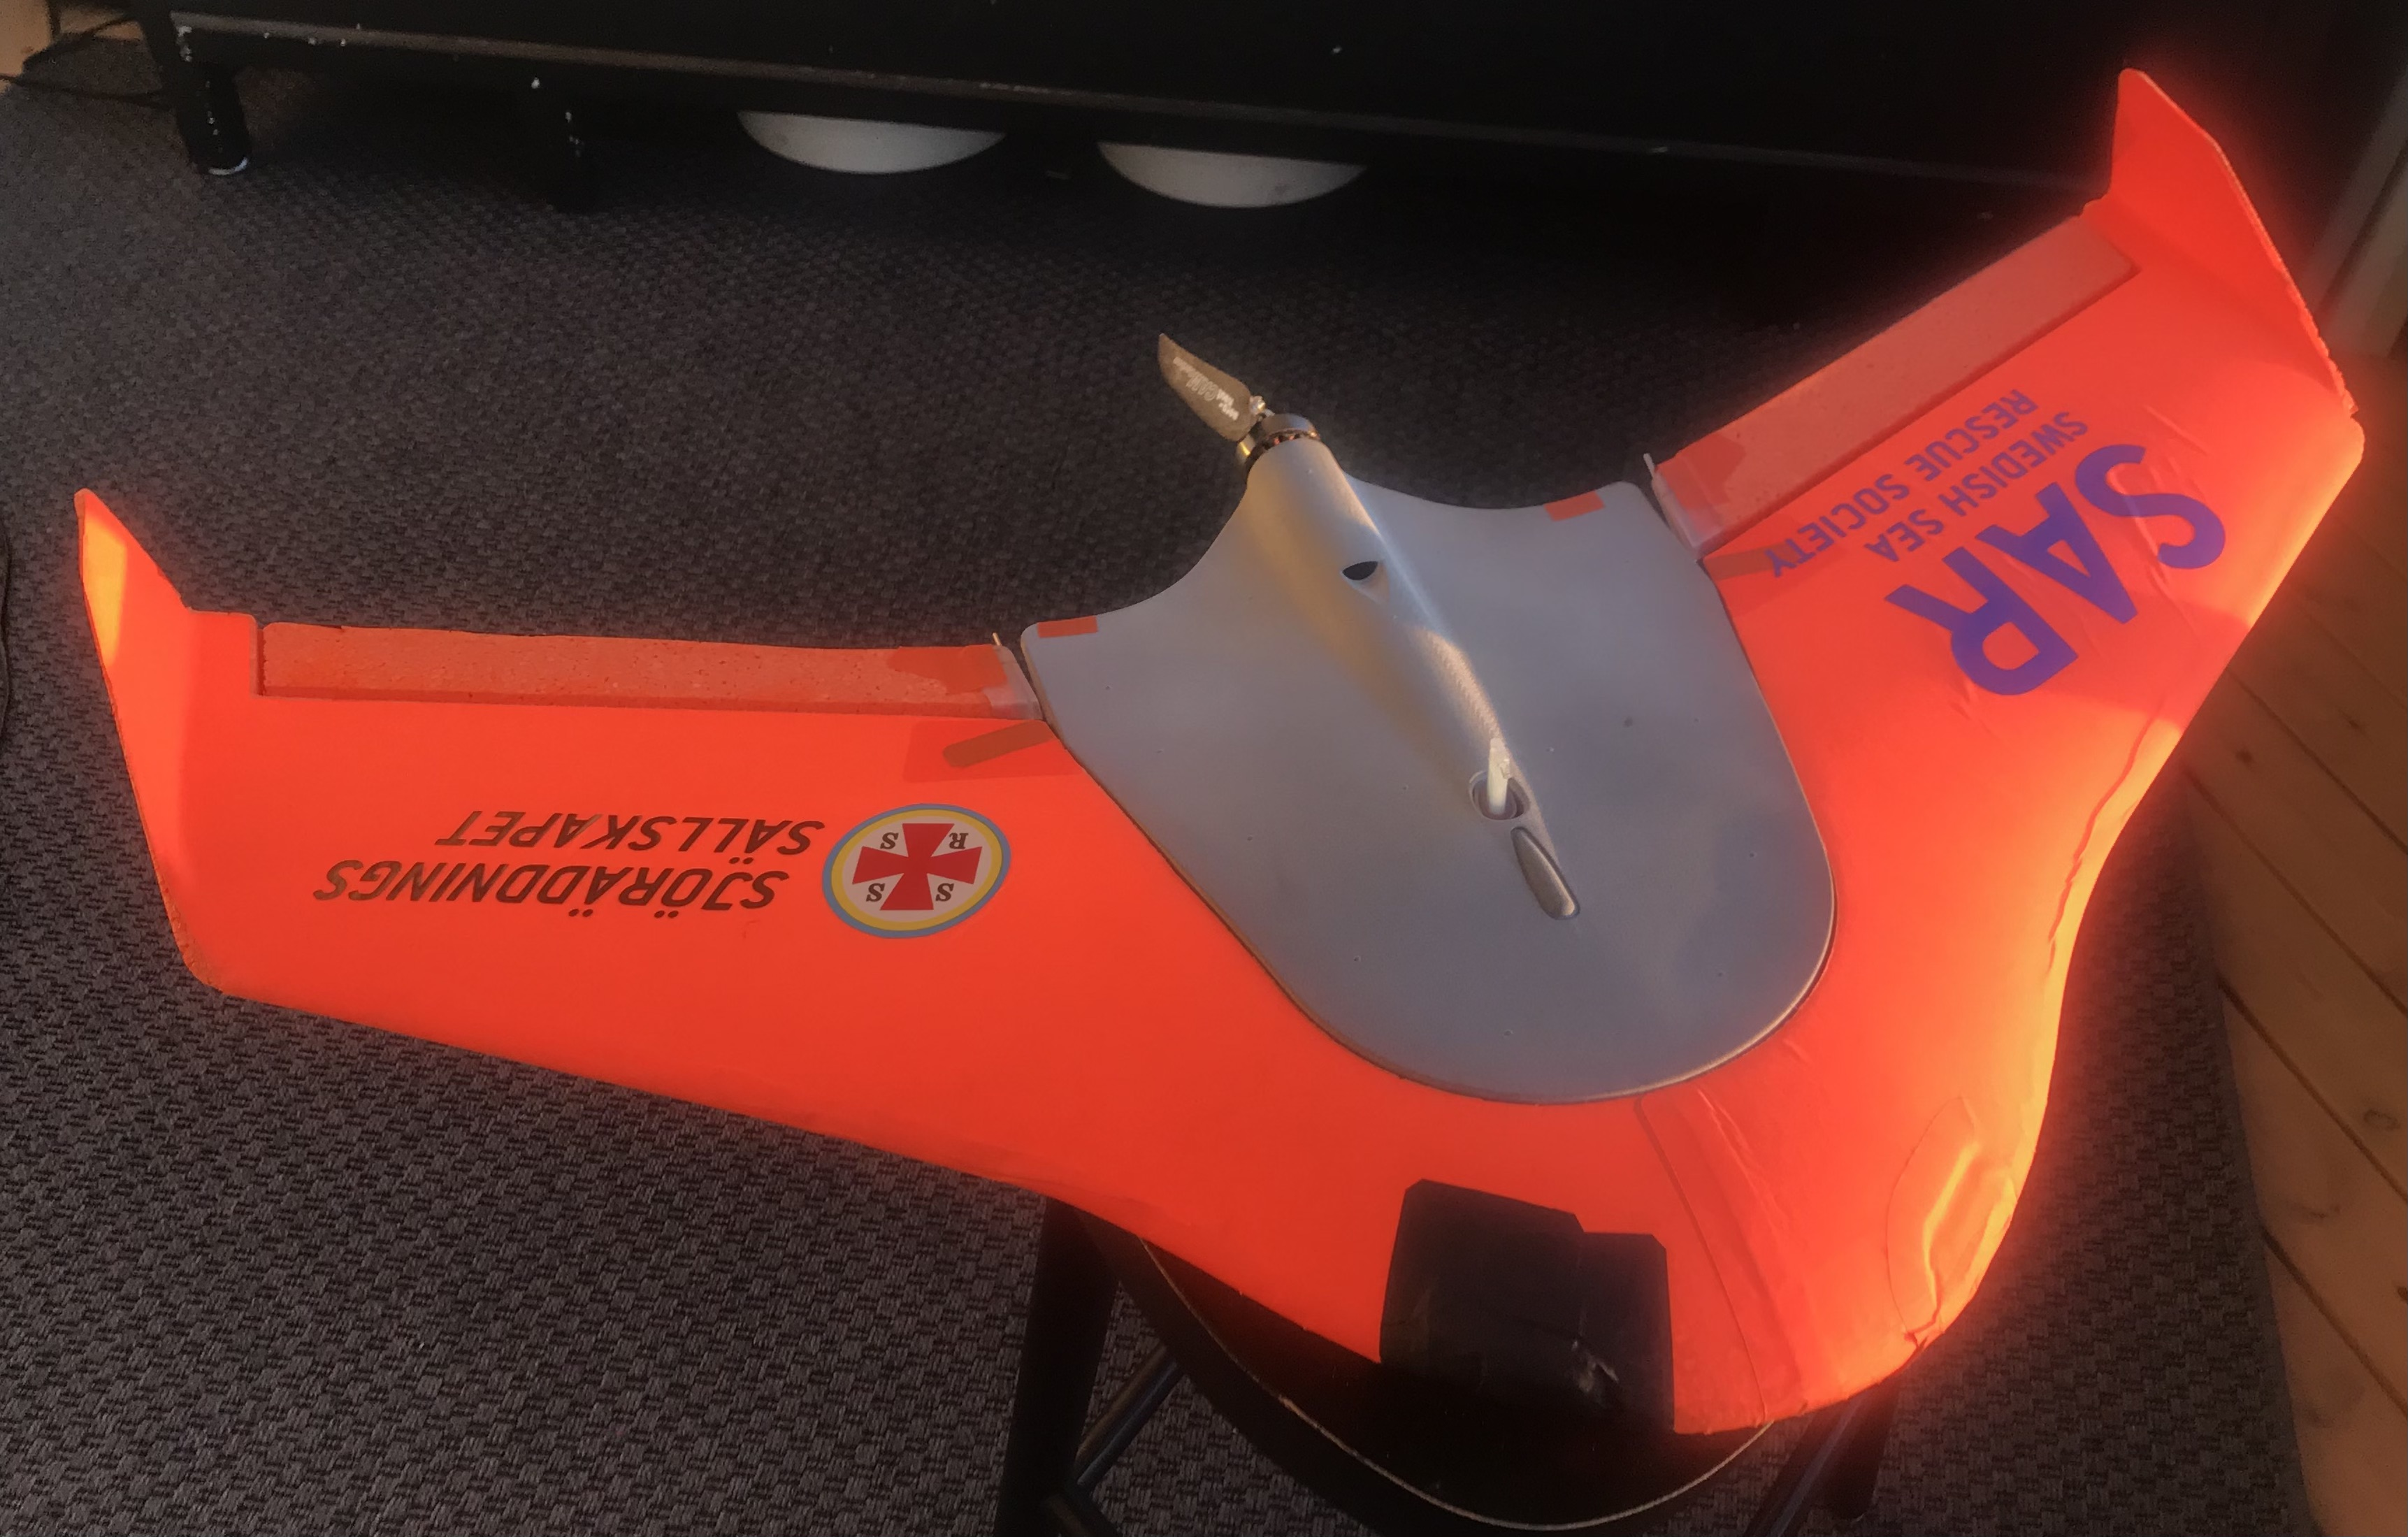
\includegraphics[width=.574\textwidth]{images/fv-3.jpg}}
   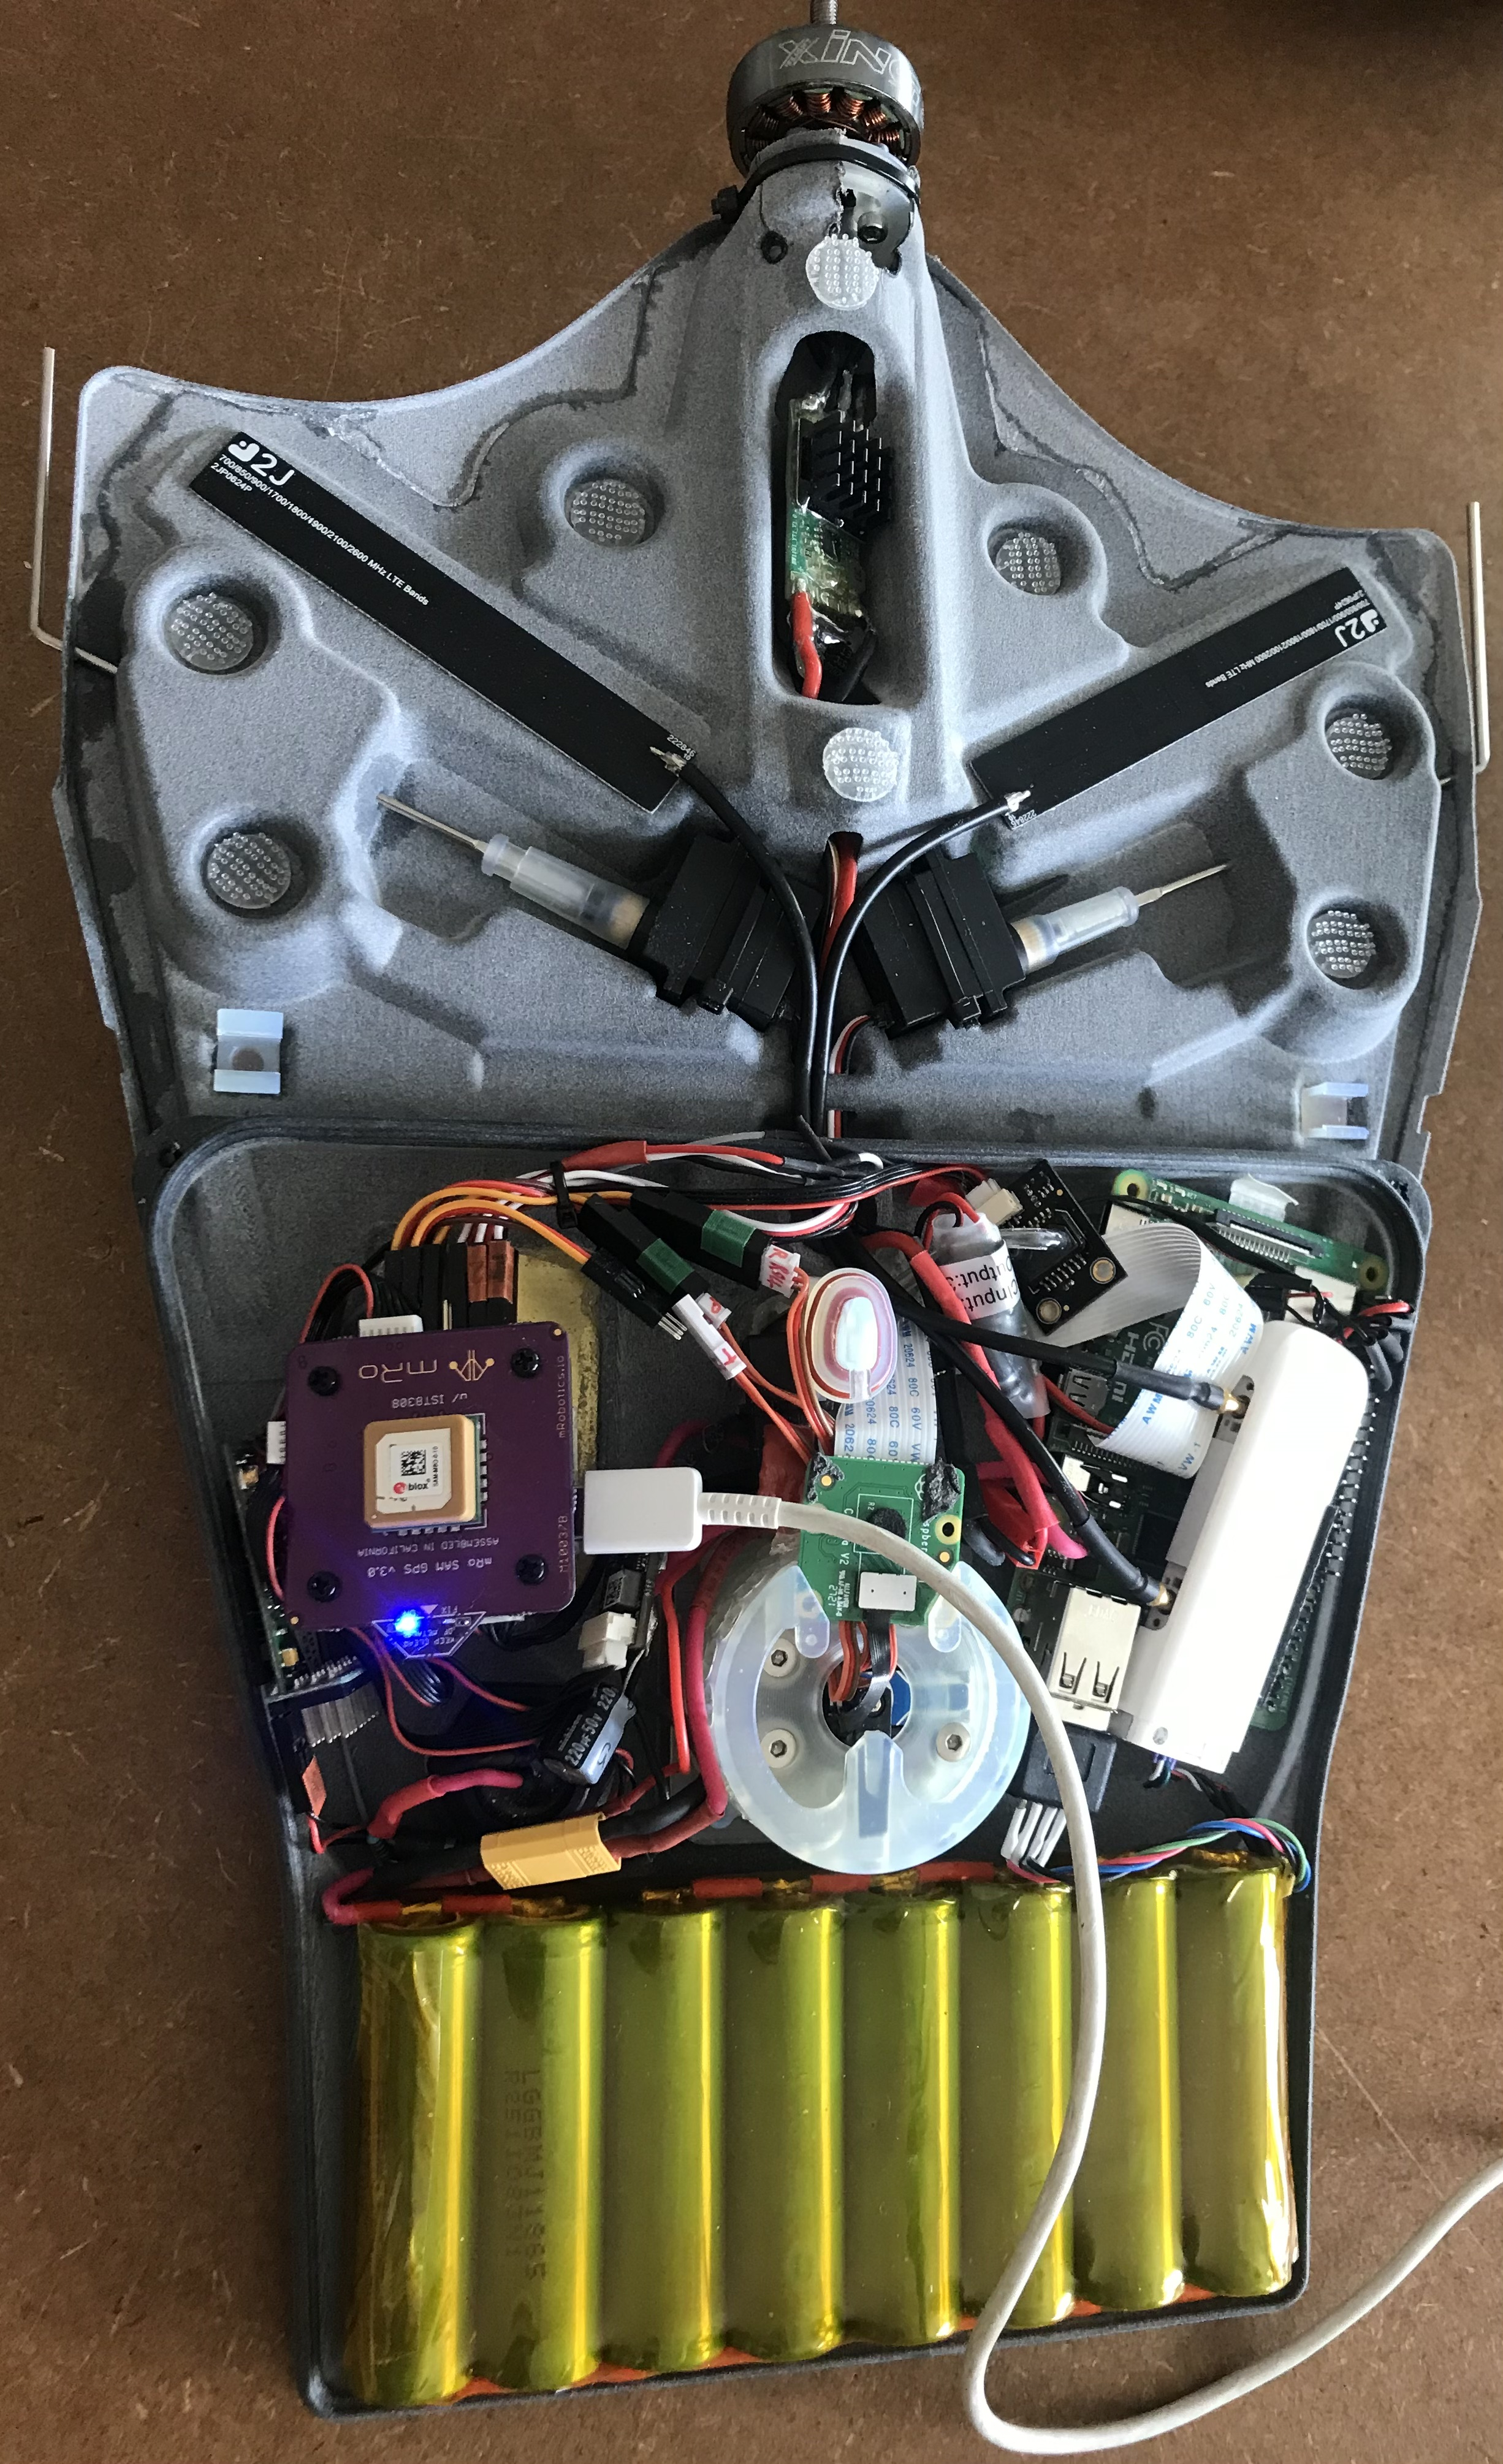
\includegraphics[width=.35\textwidth]{images/fv-1.jpg}
   \caption{The SSRS fixed-wing drone. The leftmost picture shows the full drone frame and the rightmost picture shows the inside of the drone housing with the internal components visible.}
   \label{fig:fv-drone-pics}
\end{figure}

\subsection{Fixed-wing vs. Multirotor}
Most drones used by civilians are multirotors which enable many conveniences like vertical takeoff and landing as well as stationary hovering. However, all the lift is generated by the rotors, which means that the drone needs more energy to stay in the air. Fixed-wing airframes are lifted by the downward force generated by the airflow over its' wings, which is more efficient and can thus stay in the air for longer. They are also able to travel faster as they do not need to tilt their rotors to generate forward thrust. This makes fixed-wing airframes much more suitable for long range missions, which is why it is being used in the EOS project.

\subsection{Aviation Terminology}
In aviation there are special terms for orientation used commonly when talking about the axes of the aircraft or its' equipment. In figure \ref{fig:aircraft-axes} the axes are shown for an aircraft. Roll is the rotation around the longitudinal axis, pitch is the rotation around the lateral axis and yaw is the rotation around the vertical axis. The axes are named the same when talking about the axes of the gimbal, although sometimes yaw and pitch are refered to as pan and tilt.

\begin{figure}[!hbt]
   \centering
   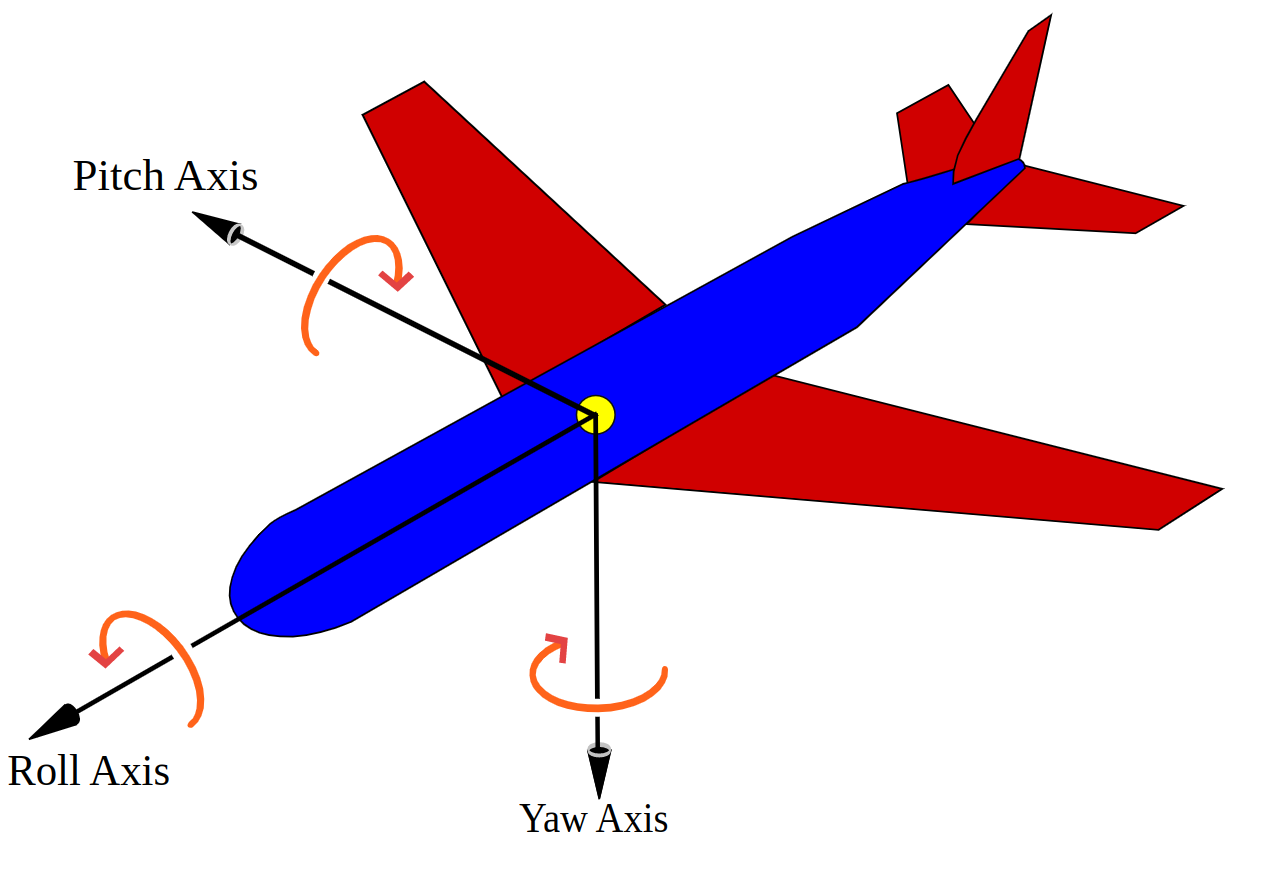
\includegraphics[scale=0.25]{images/pitch-yaw-roll.png} 
   \caption{Illustration of the roll-, pitch- and yaw-axes of an aircraft. Image credit is given to \cite{aircraft-axes-pic}.}
   \label{fig:aircraft-axes}
\end{figure}

\section{The Swedish Sea Rescue Society}
As can be read on their website \cite{ssrs}, the Swedish Sea Rescue Society (SSRS) is a non-profit organization that was founded at a conference in Stockholm in 1906 due to Sweden receiving criticism of its' poor sea rescue. Today, it is a foundation with 40 employees and over 143 000 members, and with 2400 volunteers manning their 260 rescue vessels, they carry out around 90\% of all sea rescues in Sweden all year around.

\subsection{Innovation}
As stated in their statutes \cite{ssrs-statues}, the mission of SSRS is not solely to carry out these rescue missions but to also innovate and collaborate in the area of maritime rescue as well as other aiding activities in society as a whole. As a result of this, the drone project that this thesis is a part of has been conceived along with other innovation projects such as foiling rescue boats and improved rescue vehicles \cite{surtsey-innovation}.

\section{Drone Project: Eyes On Scene}
The Eyes-On-Scene project is an innovation and research project initiated in 2021 by the SSRS, Chalmers, Infotiv, Smartplanes and Airpelago. It is partially funded by the Swedish Transport Administration as part of their airspace portfolio, and was set out to explore the possibilites of using UAVs as a support tool for sea rescue operations. A brief description of the different roles of the stakeholders are given in the following description:

\begin{description}
   \item[The Swedish Sea Rescue Society] Provide domain knowledge and requirements for the project. 
   \item[Airpelago] Develop mission control software.
   \item[Smartplanes] Develop the drone hardware.
   \item[Chalmer's University of Technology] Evaluate the project from a human factors perspective.
   \item[Infotiv] Develop the launcher used for takeoff.
\end{description}

A web interface for mission control has also been developed in the project. Currently, the interface allows flying to and loitering (circling) around waypoints given on a map where other naval and aerial traffic is displayed in real-time. The map also shows the the regulatoy zones in which one is not allowed to fly, i.e. close to airports or military zones. The interface provides video from the drone camera which is recorded and accessible after the mission.

The only way to control the direction of the camera is by providing a so-called "Region of Interest" (ROI), namely a GPS-point with latitude, longitude and altitude. The drone will then calculate the angle to the point and adjust the camera gimbal to look towards it. In the current interface it is possible to set a ROI by selecting a point on a map and uploading the new waypoint to the drone.

\section{Quality of Experience}
Quality of Experience is an emerging research field that is concerned with the user's experience in multimedia systems. It is an inherently multidisciplinary field that has close ties to the field of User Experience and Human-Computer Interaction. QoE is also closely related to the field of Quality of Service (QoS), which is concerned with the technical aspects of a system, but aims instead at evaluating the subjective experience through user experiments rather than qualitative measurements.

In the research field of QoE, common objects of study are the effects of latency, jitter or image quality on the operator's experience. Previous QoE research have been on log lifting through a VR-headset \cite{industry4.0} and remotely controlled excavation equipment \cite{latency-impact}.

In the white paper \cite{qoe-definition}, Brunström et al. make a working definition of Quality of Experience: 

\begin{quote}
   \textit{Quality of Experience (QoE) is the degree of delight or annoyance of the user of an application or service. It results from the fulfillment of his or her expectations with respect to the utility and / or enjoyment of the application or service in the light of the user’s personality and current state.} 
\end{quote}

\section{Previous Work}

W. Tärneberg et al. \cite{industry4.0} present a QoE study with industrial equipment on an excavation site where experienced operators controlled their usual equipment remotely at different latencies. They conclude that studying QoE aspects of a system is highly complex and task dependant. They also state that the operator's experience is time-variant and can be highly dependant on external factors such as lighting conditions or network quality.

K. Brunnström et al. \cite{latency-impact} performed a study on log lifting using a head-mounted display system. In the study, latency is introduced both in the display's response to movement as well as the controls. The display delay was found to have a strong effect on nausea, but an observable effect on controller latency could only be found at latencies above 800 ms. 

As part of the Eyes-On-Scene-project, a study was performed at Chalmers by Grote et al. \cite{eos-maritime} where two maritime emergency calls were performed, one with and one without images from a UAV at the emergency site. The study showed that imagery from the accident gave the rescue personnel a sense of control before arriving at the scene when knowing what they were going to face. The crew was also faster at locating a person or object when having aerial footage of the scene.

In \cite{targetting}, M. Quigley et al. present a test bed with a fixed-wing UAV on which they evaluate different means of gimbal control. They find that altitude estimation causes problems with ROI-control, which results in the gimbal pointing at a circle around the point instead of directly at it. To address this they introduce controls for changing the altitude as well as the coordinates of the point, and they also have a mode in which the plane updates it's loiter point to where the gimbal is looking. Manual controls of the gimbal are also implemented using a game controller. In their test bed they map the left joystick to the attitude control of the aircraft while the right joystick is mapped to different states of the gimbal, instead of relative position.

\section{Pre-existing Hardware}
In this section the hardware used in the experiments is presented.

\subsection{Fixed-Wing Drone}
\label{sec:uav-components}
The drone components relevant for this thesis are detailed in the following description. Pictures of the drone can be seen in \ref{fig:fv-drone-pics} and explanation of its' design is described in section \ref{sec:fixed-wing-uav}.

\begin{description}
   \item[Flight Controller: Pixracer R15] The flight controller is the brain of the aircraft and houses components and connectors relevant to in-flight operations such as servos for control surfaces or other equipment, GPS and accelorometer.

   \item[Companion Computer: Raspberry Pi 4] The Raspberry Pi serves as the onboard computer, commonly known as the "companion computer" in the context of drone hardware. It is connected to the flight controller via USB and makes it possible to relay messages sent over ethernet instead of radio, allowing to connect to a ground station over the Internet. 
   
   \item[4G Modem] Sim-card modem allowing access to the mobile network. 
   
   \item[Raspberry Pi Camera Module v2] The camera module is a small camera that is mounted inside on a flat surface on the gimbal. The camera connects to the module board which is then connected to the Raspberry Pi with a ribbon cable. It is capable of recording 1440x1080 video at 30 fps and has a 4:3 aspect ration. 

   \item[Camera Gimbal] The camera gimbal on the drone is designed and manufactured by Fredrik Falkman at the SSRS. It is a 3D-printed design that has three degrees of freedom made possible by three servos connected to drive belts that control each axis of the camera. The servos are connected to the flight controller which also provide them with power. The gimbal is designed to house a small camera which when mounted looks out from the bottom of the drone. In \ref{fig:gimbal-pics} the schematics of the gimbal can be seen. 
   
   \begin{figure}[htp]
      \centering
      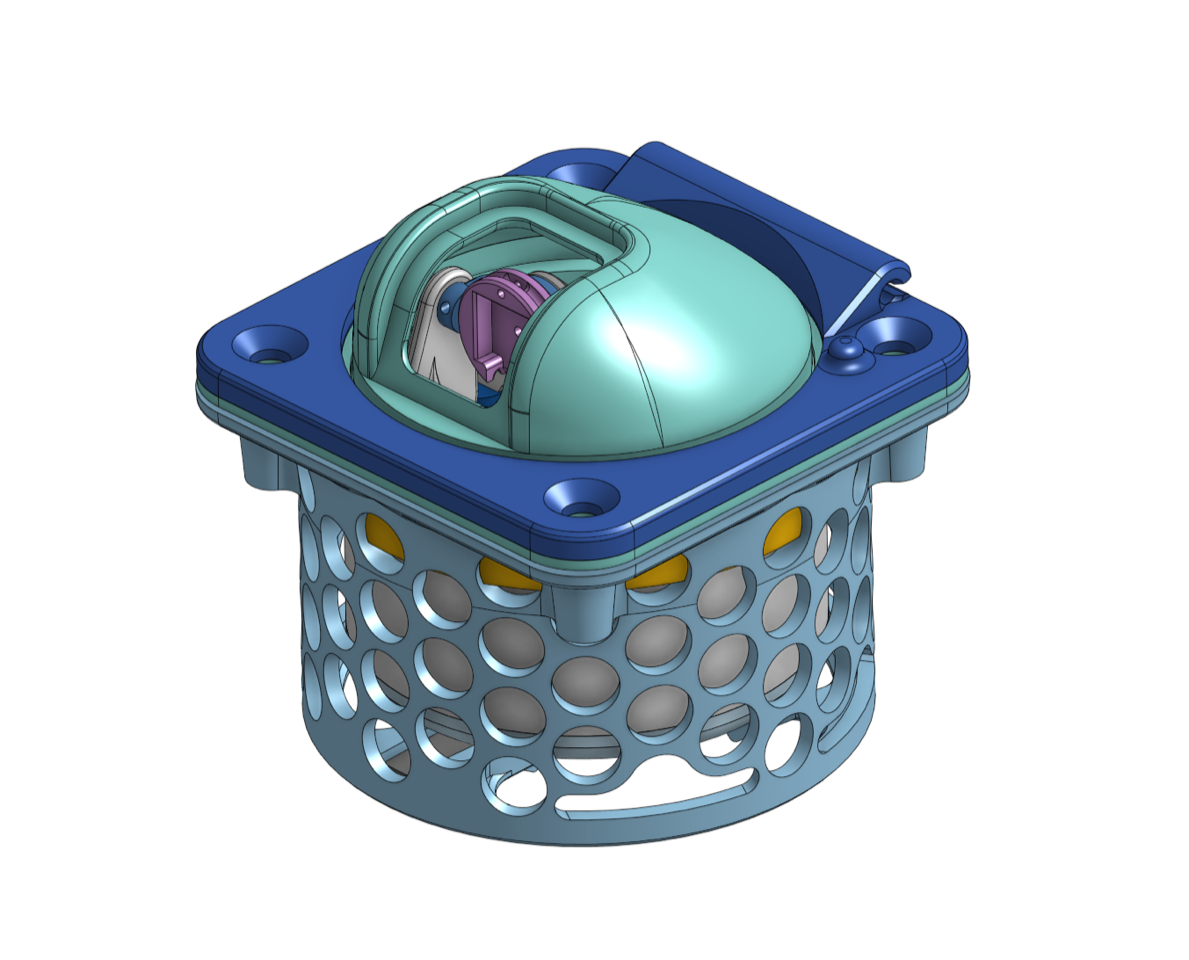
\includegraphics[width=.3\textwidth]{images/gimbal-1.png}\hfill
      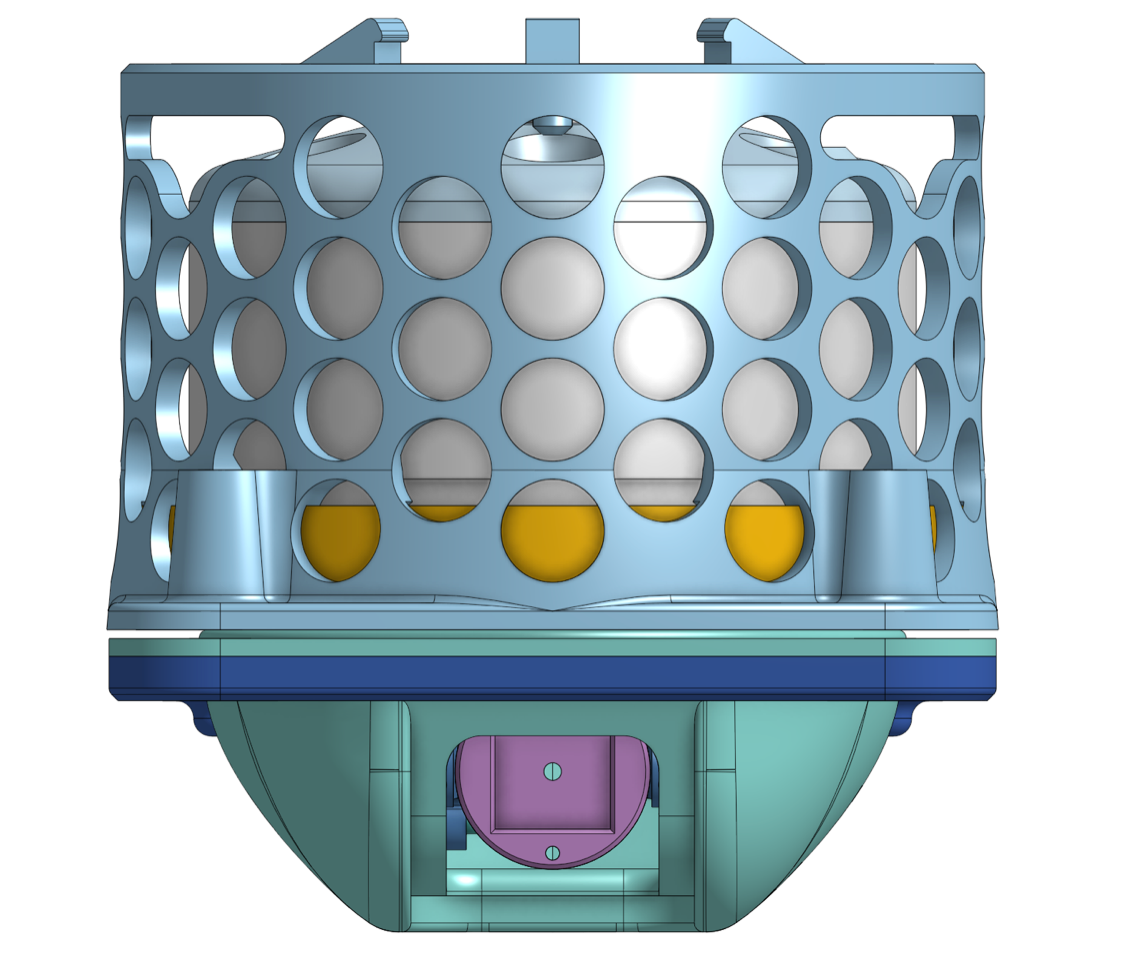
\includegraphics[width=.3\textwidth]{images/gimbal-2.png}\hfill
      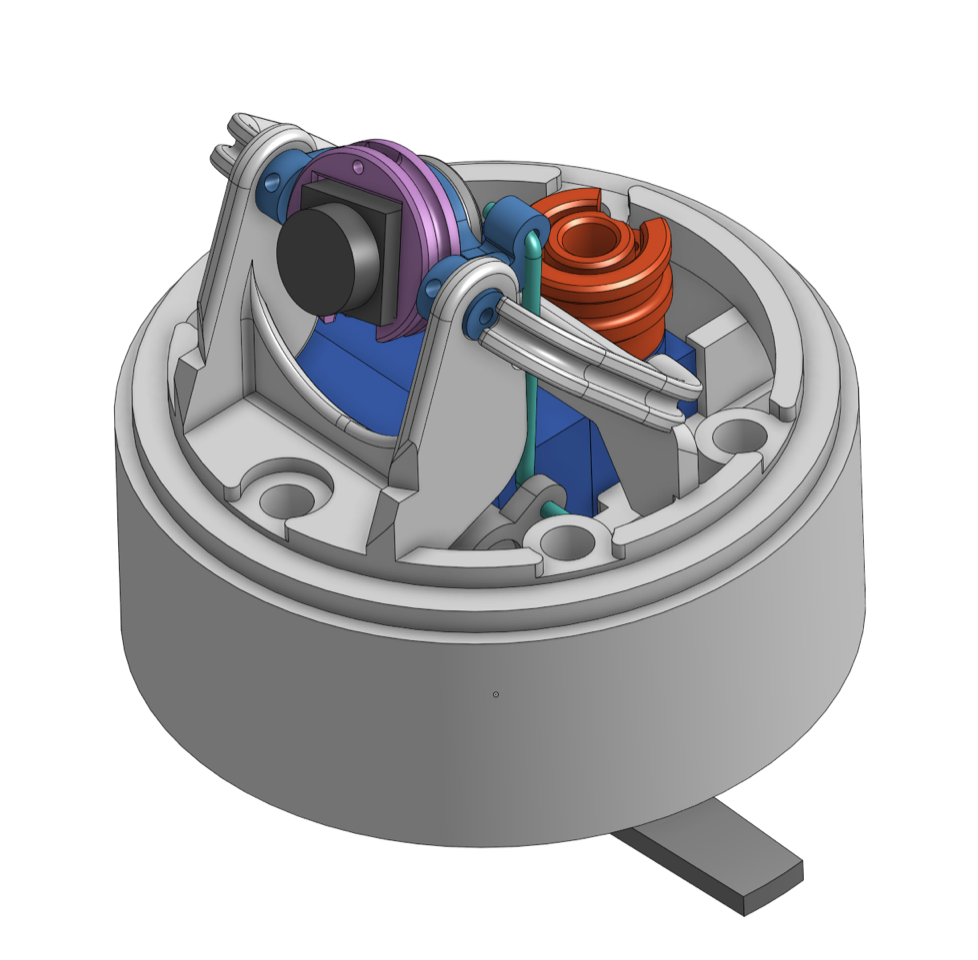
\includegraphics[width=.3\textwidth]{images/gimbal-3.png}
      \caption{Schematics of the drone gimbal. The middle and left picture shows the gimbal with its full housing. To the right the housing has has been removed and a mockup camera module has been inserted on the mounting plate.}
      \label{fig:gimbal-pics}
   \end{figure}
\end{description}
   
\subsection{Hoverboard robot}
In order to introduce movement in the QoE experiment, a modified hoverboard was used. The hoverboard has four wheels and could be controlled via joystick inputs or coordinates. It's manouvering was assisted by real-time lidar-mapping of the room. The hoverboard can be seen in \ref{fig:hoverboard}

\begin{figure}[!hbt]
   \centering
   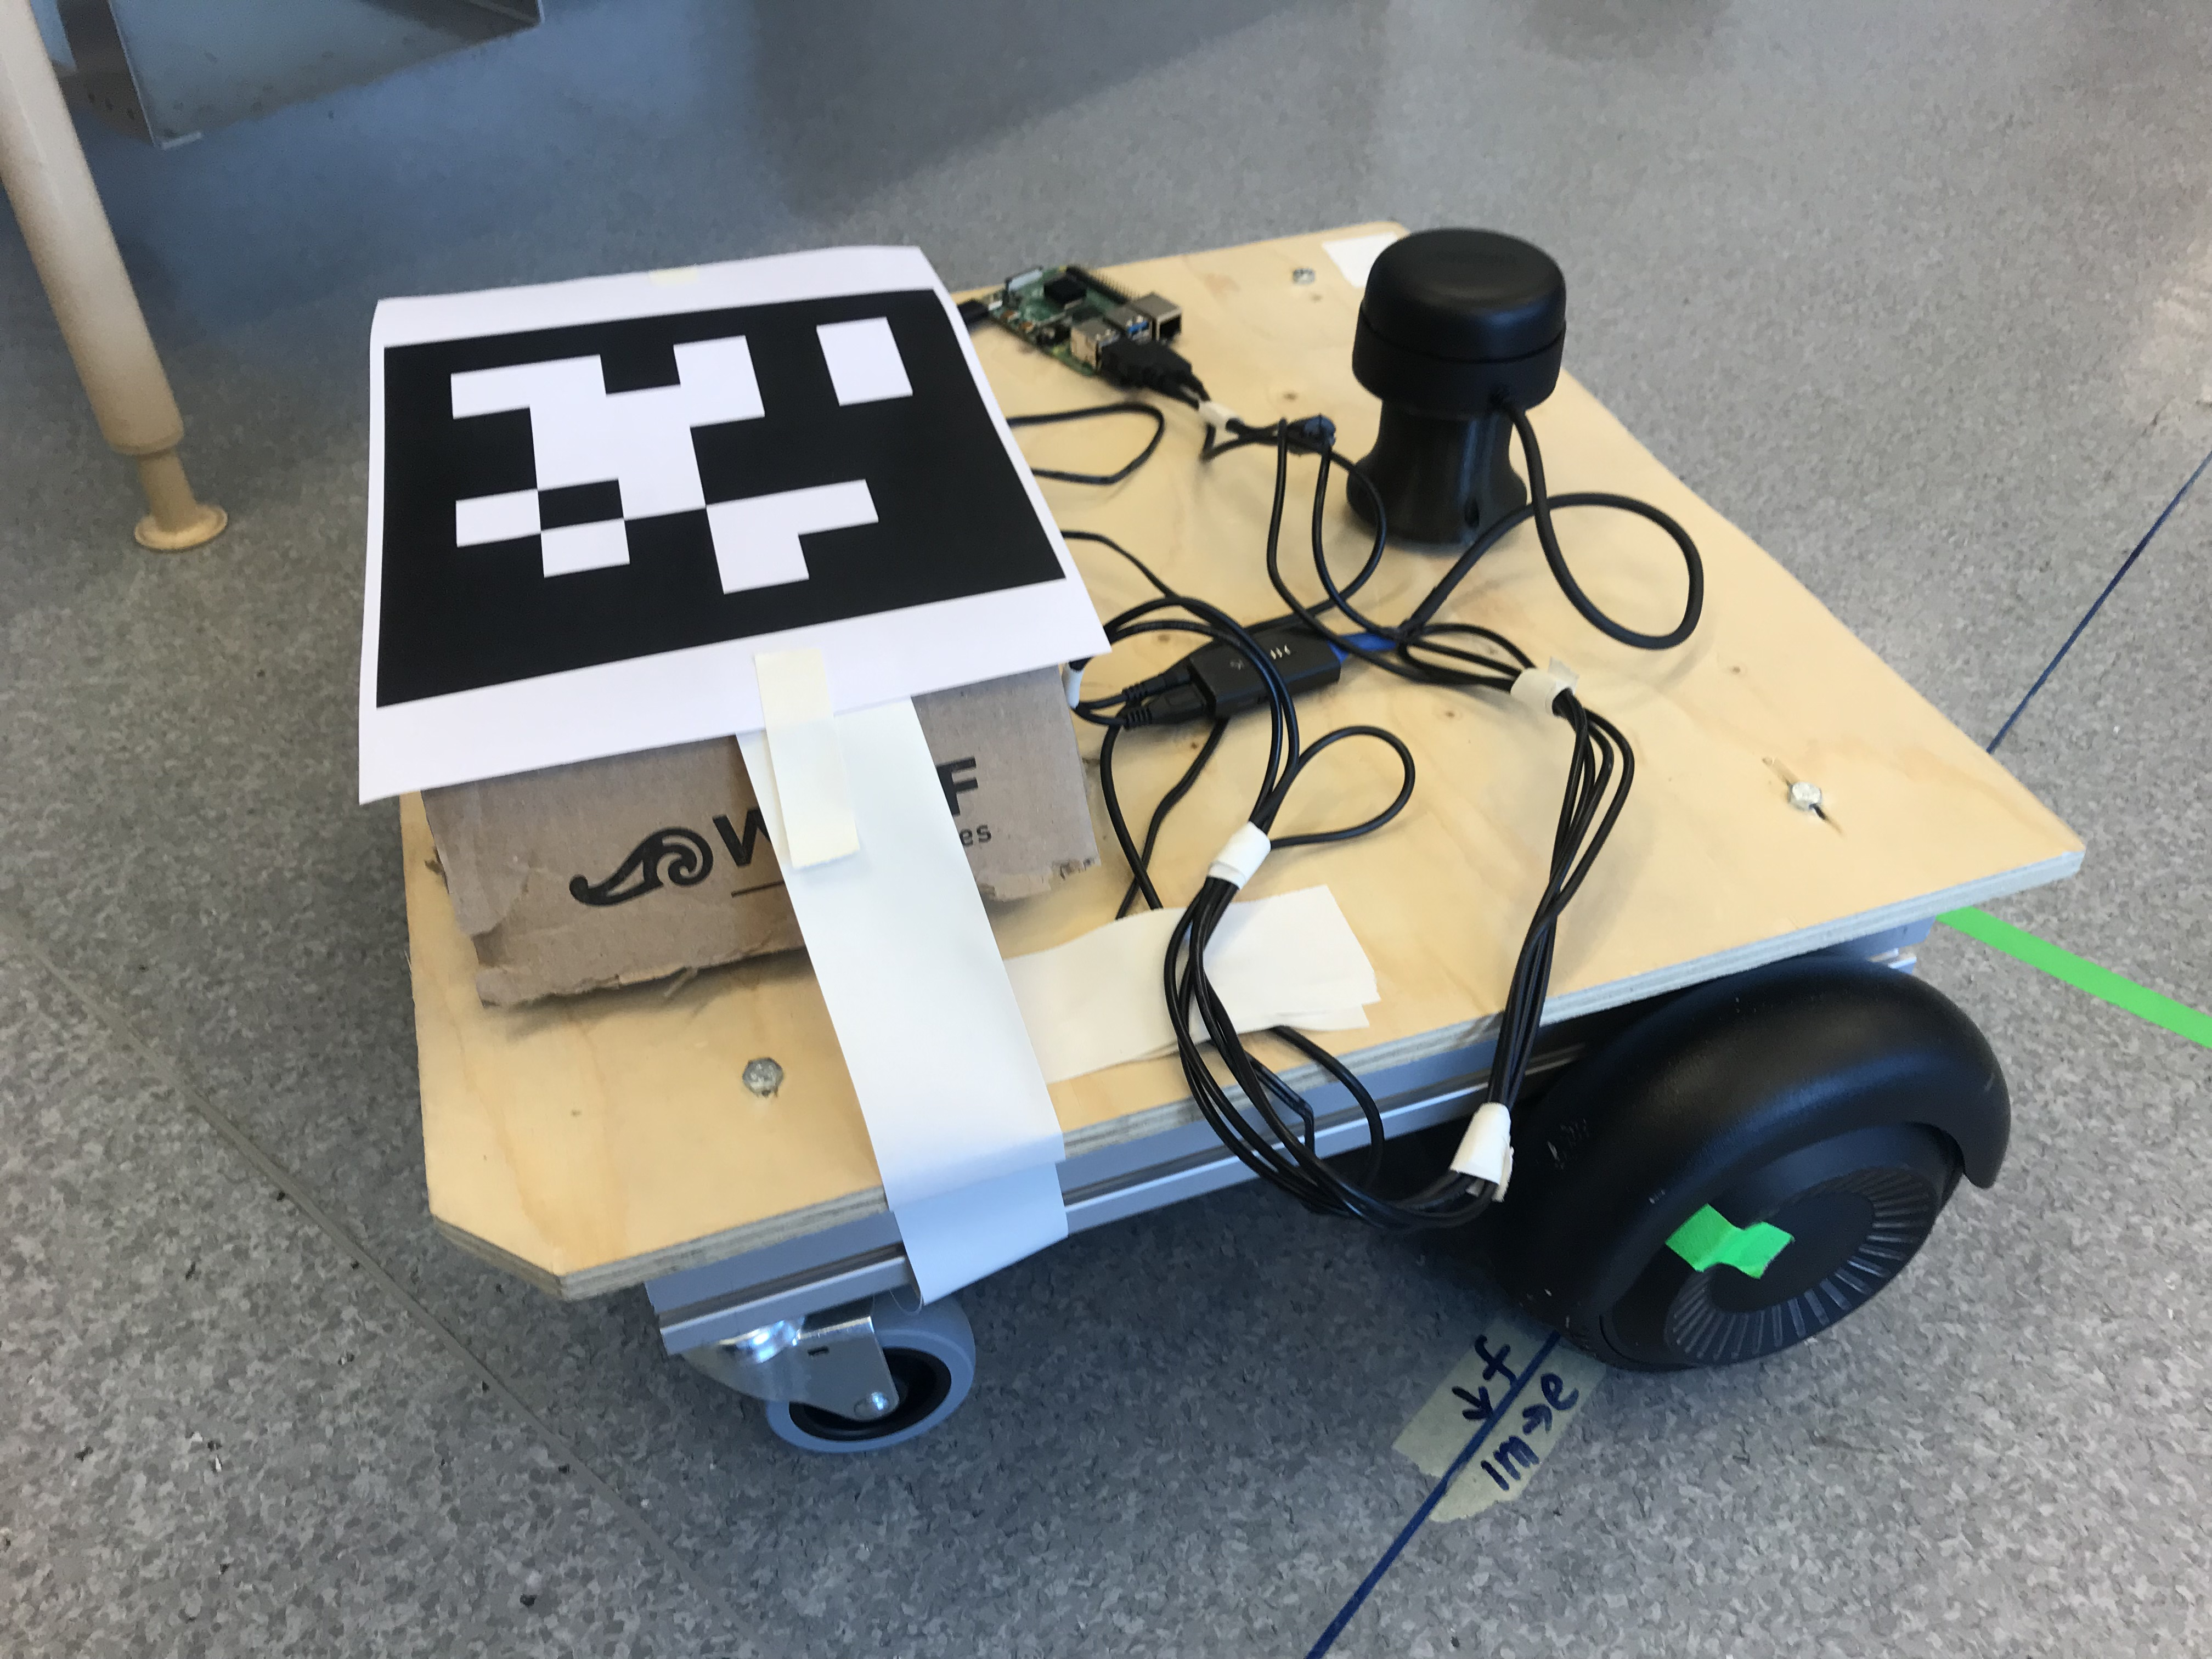
\includegraphics[scale=0.07]{images/hoverboard.jpg} 
   \caption{}
   \label{fig:hoverboard}
\end{figure}

The average velocity of the hoverboard was determined at 0.184 m/s with a standard deviation of 0.0062 m/s. The error after each lap is presented in table \ref{tab:hoverboard-error}, and was non accumulative over multiple laps. 

\begin{table}[!hbt]
   \centering
   \label{tab:hoverboard-error}
   \begin{tabular}{|c|c|c|c|}
      \hline
      \textbf{Axis} & \textbf{Average (mm)} & \textbf{Min (mm)} & \textbf{Max(mm)} \\
      \hline
      $x$ & $6.8 $ & $-40.2$ & $51$ \\
      \hline
      $y$ & $42.78$ & $34.9$ & $50.9$ \\
      \hline
   \end{tabular}
\end{table}

\subsection{Apriltag}
An apriltag is a type of low-resolution QR-code often used in robotics to estimate orientation and position of robots or objects with the help of computer vision. It was fastened on top of the hoverboard as high as possible without blocking the lidar. The apriltag can be seen mounted on the hoverboard in figure \ref{fig:hoverboard}.

\section{Pre-existing Software}
In this section the already finished software used in the experiments will be detailed.

\begin{description}
   \item[Firmware: ArduPlane]
   The firmware running on the flight controller is called ArduPlane, which is part of the open-source autopilot software suite ArduPilot that enables the creation of unmanned, autonomous vehicles \cite{ardupilot-org}. It is developed by a community of developers and is available on GitHub \cite{ardupilot-github}.
   
   \item[Protocol: MAVLink]
   As can be read on their website \cite{mavlink}, MAVLink is a lightweight protocol suited for communication with drones and between drone components. It has a byte overhead of 14 bytes and allows for concurrent communication between up to 255 systems. 

   \item [Software: MAVProxy]
   MAVProxy \cite{mavproxy} is a software running on the companion computer whose task is to relay MAVLink messages from an ethernet interface to the flight controllers serial interface. 

   \item[UV4L]
   UV4L is a video streaming server that supports several real-time communication protocols and video encodings \cite{uv4l}. It's function in the test bed is to stream the video from the camera to the web. As for video encoding, MJPEG was used.
   
   \item[Janus Server]
   As described on their webpage \cite{janus}, Janus is a plugin-based software that helps establish WebRTC connections. In this thesis it is used to establish the connection between the UV4L server and the web browser, enabling the peer-to-peer connection between the two devices.

   \item[Hoverboard software] The hoverboard has software which allows it to be controlled by a game controller or follow a set of points using coordinates for which it uses it's Lidar and a SLAM-algorithm. This makes it possible to have the hoverboard run in a programmed route with little error. 
\end{description}

\chapter{Implementation of Test Bed}
In this chapter the hardware and software developed specifically for the thesis will be detailed.

\section{Gimbal Box}
As the entire drone was not needed to conduct the QoE experiment, a Raspberry Pi, flight controller and gimbal were mounted inside a 2L Ikea SmartStore box. The computer boards were mounted inside the box with velcro tape and the gimbal was mounted in a cutout in the bottom of the box. Pictures of the box can be seen in figure \ref{fig:drone-setup}.

\begin{figure}[htp]
   \centering
   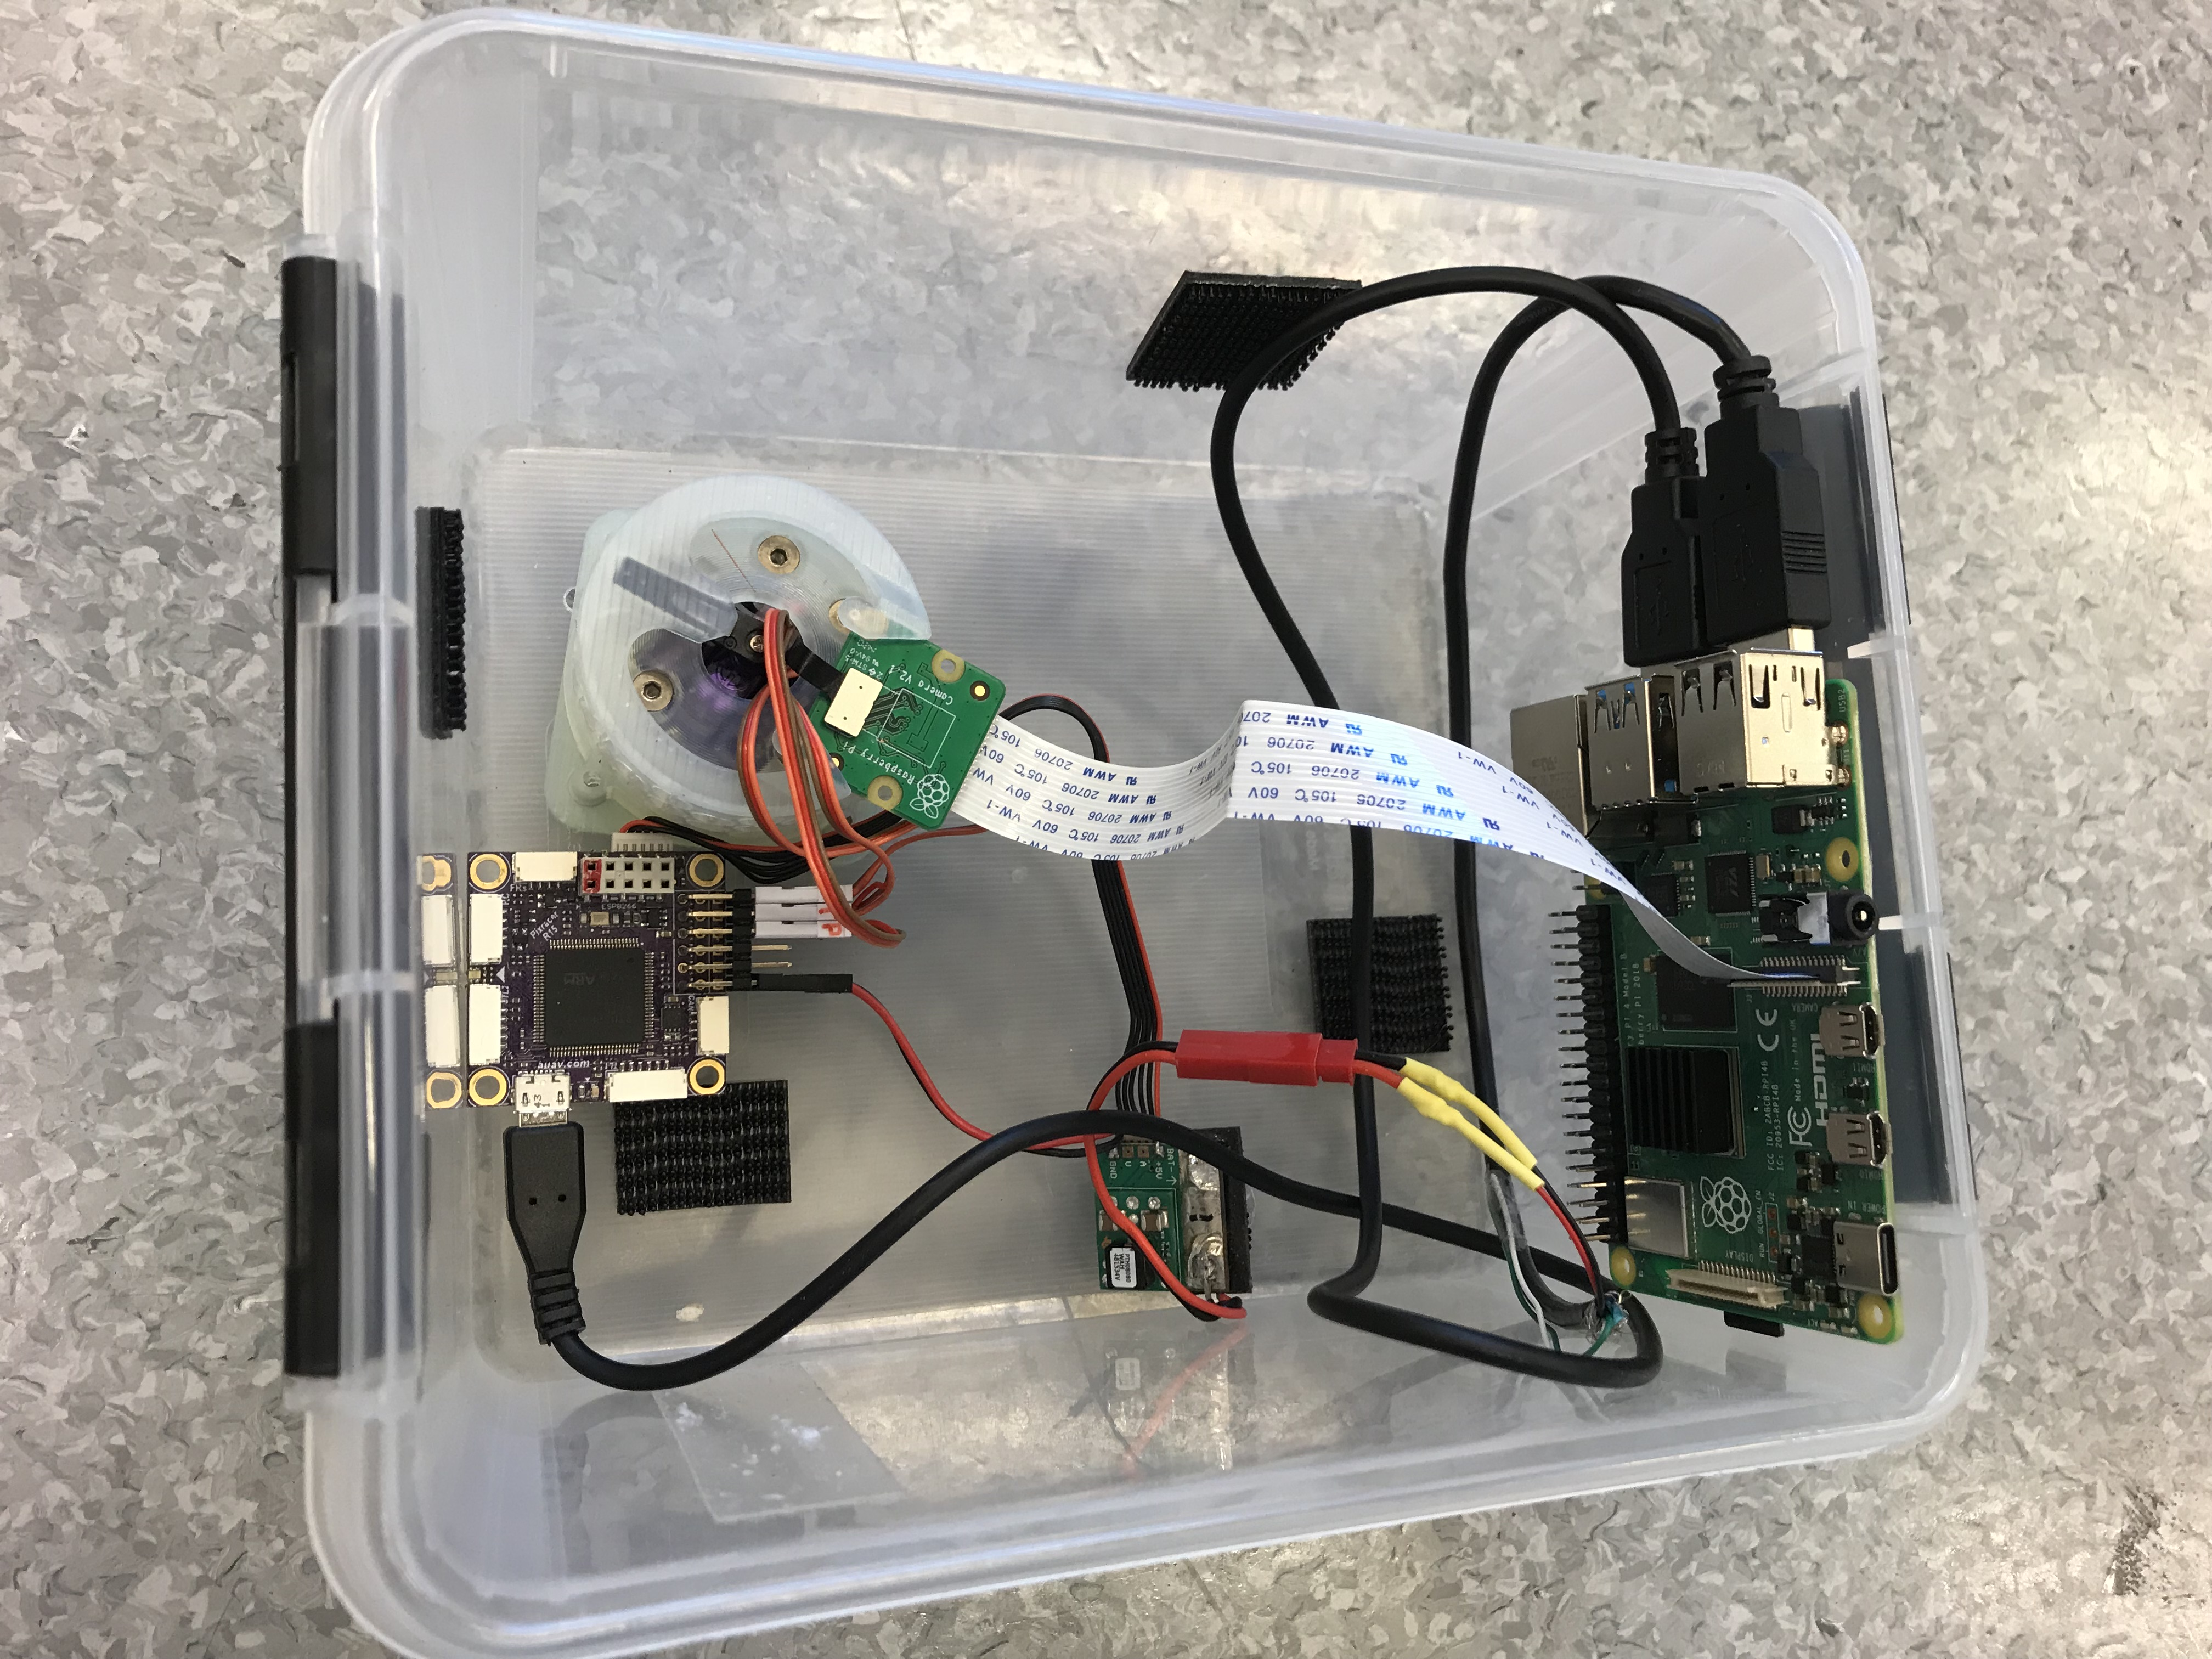
\includegraphics[width=.47\textwidth]{images/drone-box-1.jpg}\hfill
   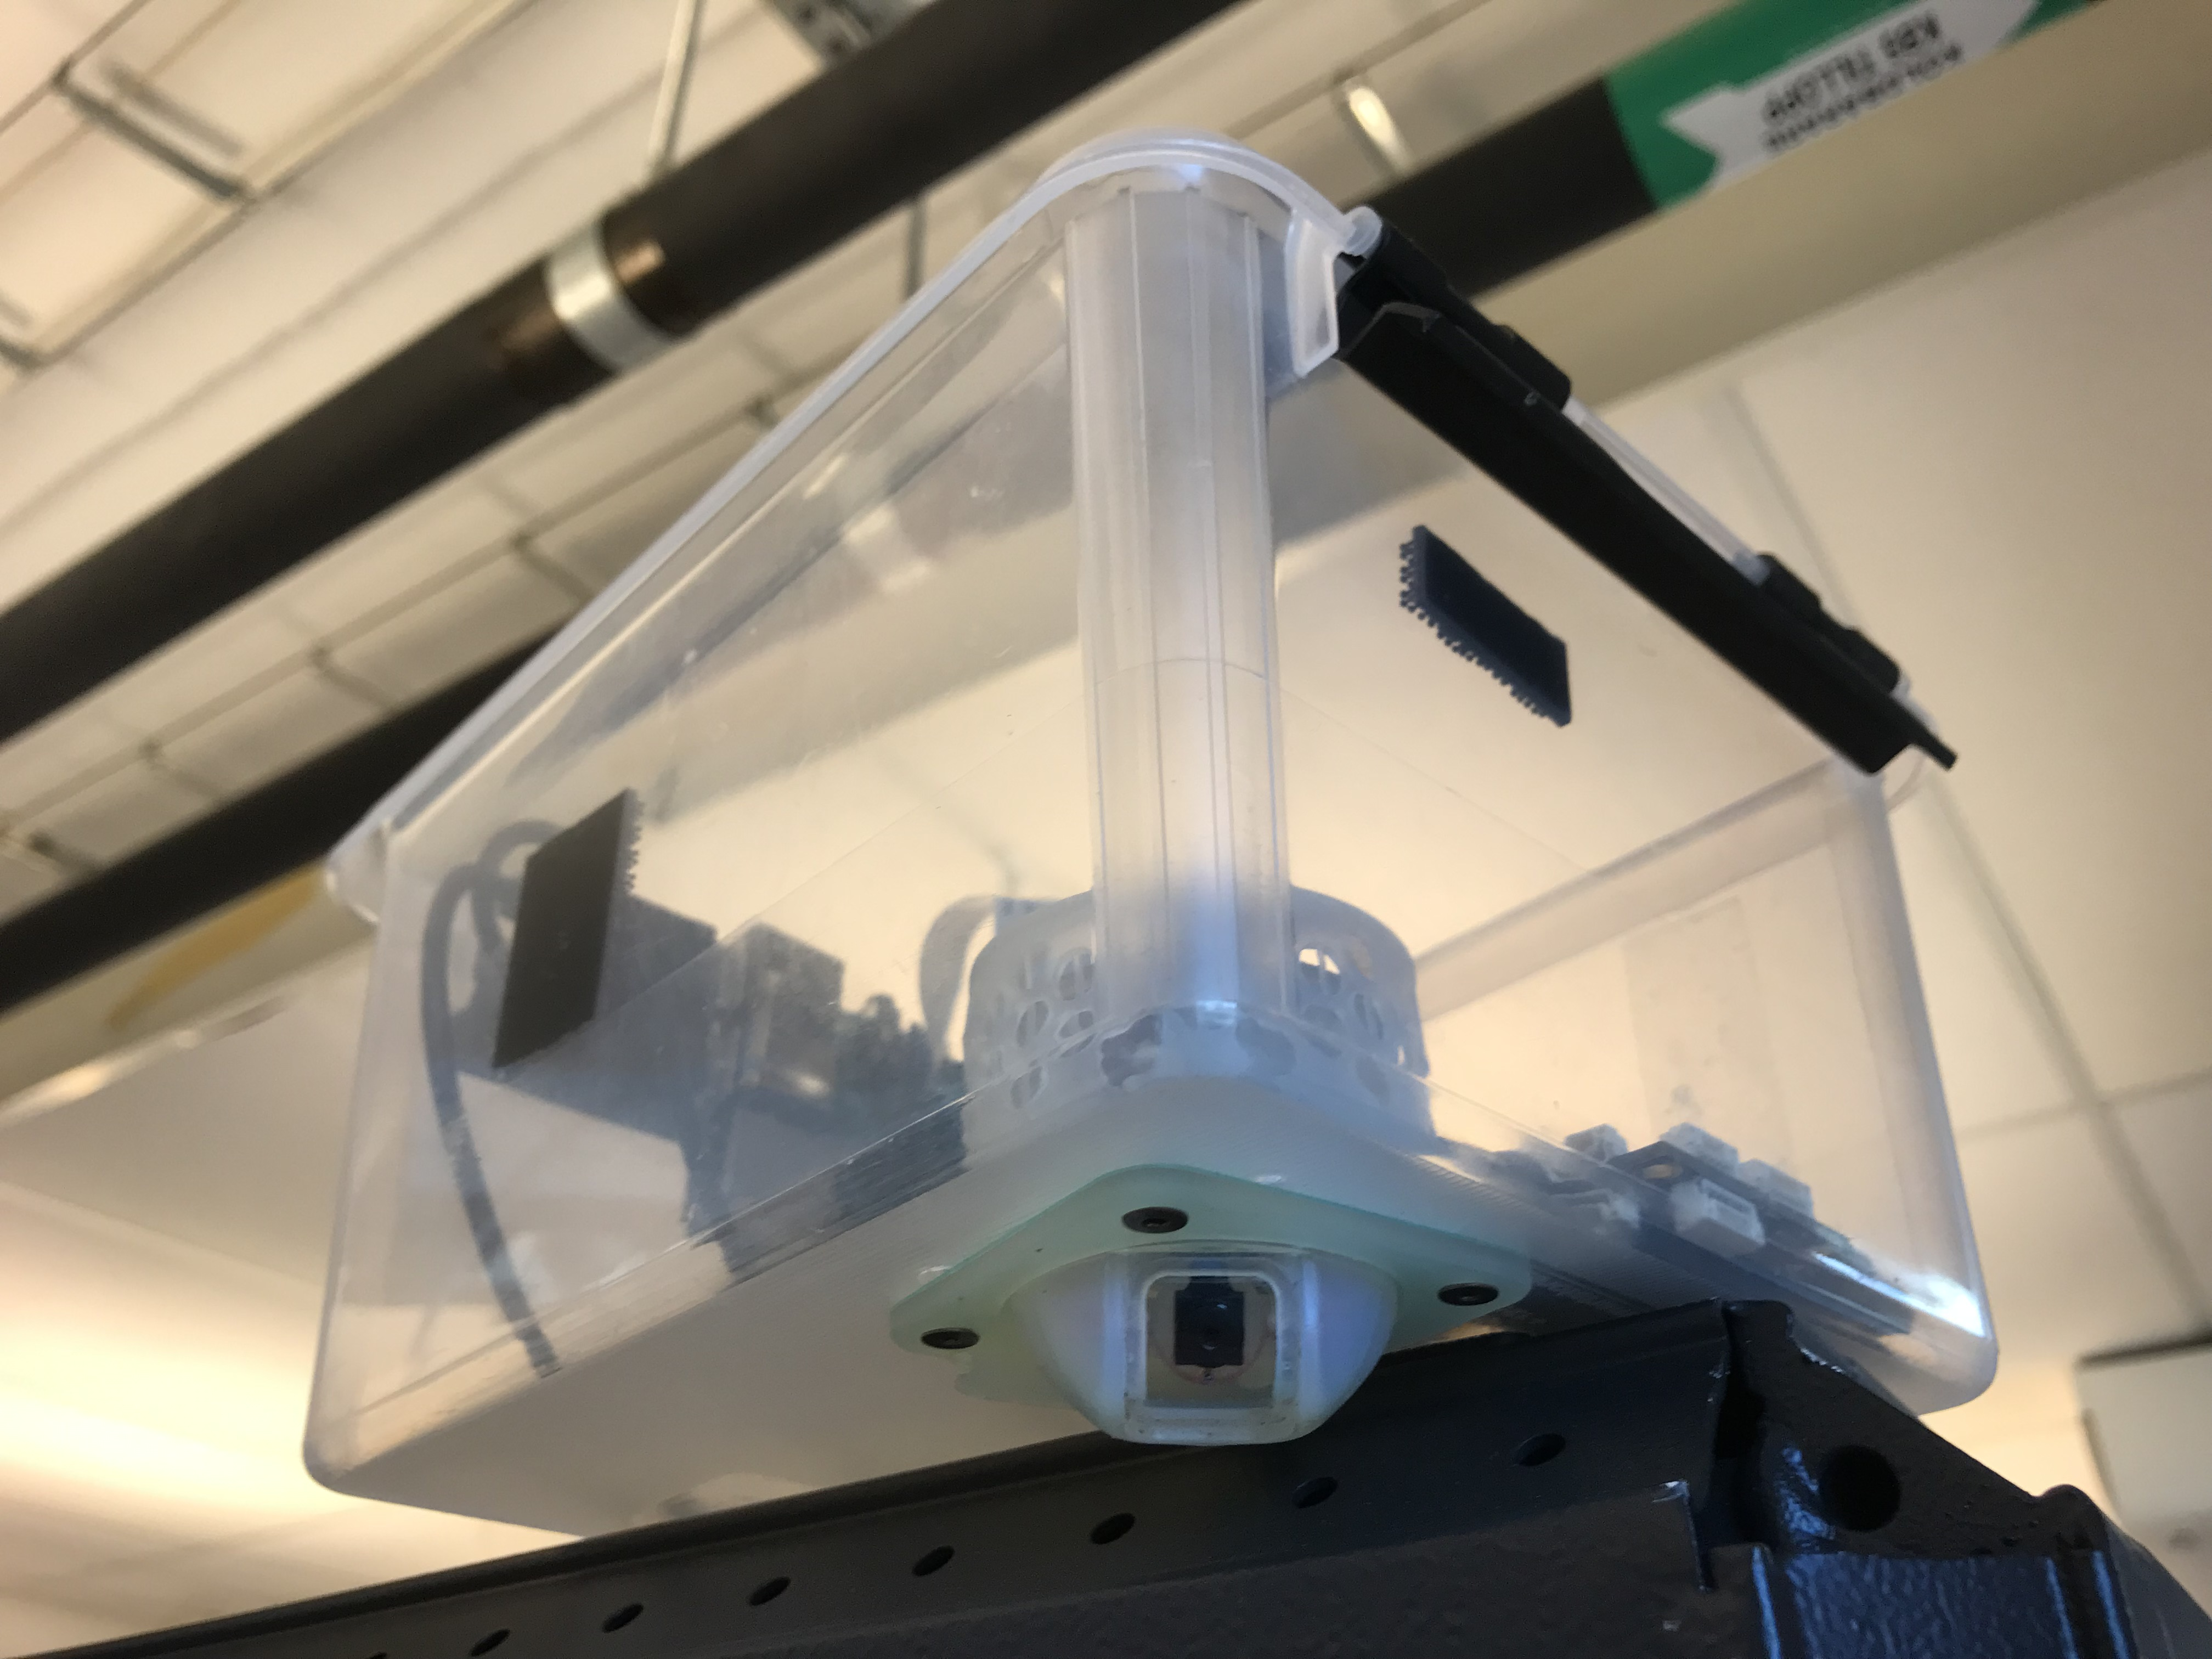
\includegraphics[width=.47\textwidth]{images/drone-box-2.jpg}
   \caption{The box that houses the drone hardware for the experiment. The left picture shows the box from above, from the left the following components are visible: flight controller, gimbal with camera module, power supply and Raspberry Pi. The right image shows the box from below.}
   \label{fig:drone-setup}
\end{figure}


\section{Gimbal Control Interface}
Addressing goal \textbf{G1} of the thesis, a program was implemented in Python displaying the video feed from the drone camera while taking control inputs from the operator. The inputs came from the right joystick of a PlayStation-controller while the program sent messages updating the gimbal's position with a set frequency. The program could also record the video feed displayed to the gimbal operator. A visual overview of the system is shown in Figure \ref{fig:system-overview}.
\begin{figure}[!hbt]
   \centering
   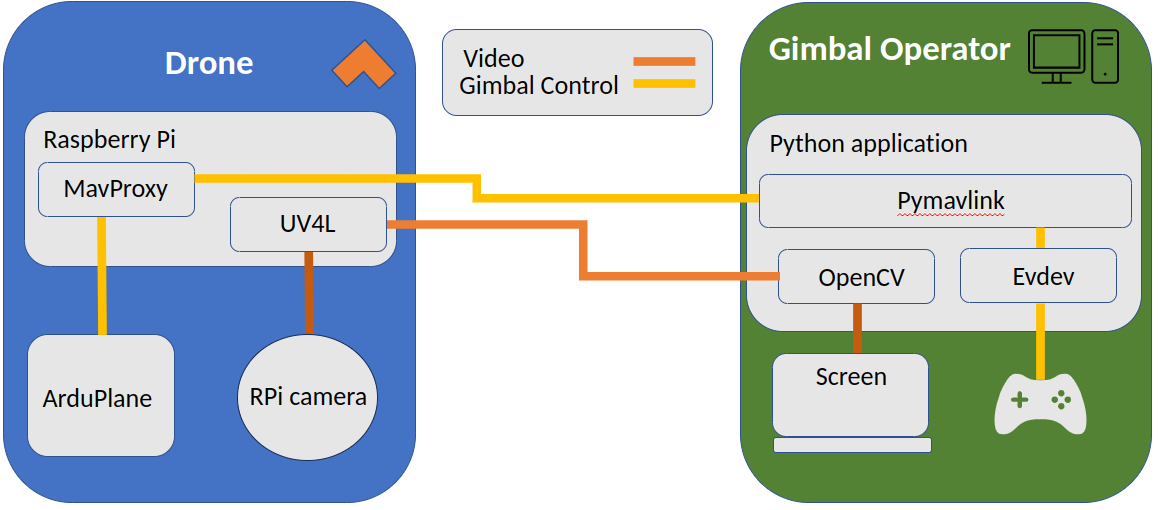
\includegraphics[scale=0.5]{images/system-overview.png} 
   \caption{An overview of the entire system. On the left, the drone and it's components including the RPi, RPi camera module and the flight controller are shown. On the right, the ground station and its' components including the web application, Janus server and the controller are shown. The colour of the connections represent what data they transfer, where orange is video, orange double-line is video negotiation and yellow is control.}
   \label{fig:system-overview}
\end{figure}

The application was run with Python version 3.9.16 and used the following libraries:
\begin{description} 
   \item [pymavlink (v. 2.4.37)]
   An interface to communicate with MAVLink devices, available at \cite{pymavlink}. With the library a port can be set to send and receive MAVLink messages.
 
   \item [Evdev v. (1.6.1)]
   A python library for interrupt-driven input devices. It is used for reading input from the Playstation-controller. Available at \cite{evdev}.

   \item [OpenCV (v. 4.7)] 
   Open Computer Vision, a very popular library for video and computer vision tasks. In the test interface it is used for displaying and recording the video feed. Available at \cite{opencv}.

   \item[Multiprocessing]
   This standard module was used in order to run the video tasks in different processes to not interfere with the control. The video frames were accessed and displayed by one process and then feeded to another process saving each frame. For more information on the library see \cite{multiprocessing}.  
\end{description}

\subsection{Delay}

Delay in the controls could be introduced by providing a program argument. The delay was simulated by putting each outgoing message in a queue along with a timestamp, with the program waiting until \ timestamp + delay \ was reached before sending the command. The following algorithm was used to schedule the sending of commands according to the delay:
\begin{algorithmic}
   \While{running}
   \State $timestamp, pitch, yaw = queue.get()$ // blocking call
   \State $t_{0} = time.now$
   \State $diff = timestamp + delay - t_{0}$
   \If{diff > 0}
      \State $time.sleep(diff)$
   \EndIf
   \State $drone\_connection.send\_pitch\_yaw(pitch, yaw)$
   \EndWhile
\end{algorithmic}

The screen and the controller were then filmed on a phone in 120 FPS to measure the time between a control input to the video feed updating. To measure the network delay a simple ping-measure was taken.

The network latency was found to be below 1 ms. The delay of the video feed alone was between 100-150ms while the full controller to video feedback delay was around 400ms. 

\subsection{Sources of Delay}
Although the sources of the delay were not examined in any great depth some probable causes were:
\begin{description}
   \item[Message frequency] 
   While the internal model of the gimbal's orientation was updated by interrupts, the message rate to the flight controller was set to a maximum of 20Hz, resulting in a delay between 0-50ms for each message.
   
   \item [Video encoding]
   The delay of the video feed was measured by recording a stopwatch, the controller and the video feed of the stopwatch simultaneously. The difference between the stopwatch on the recording and the screen was estimated to be between 100-150ms.
   
   \item [Network delay] 
   The network delay was measured with pings to be below 1ms. 

   \item[MAVProxy relaying] Each message must be taken from the ethernet interface of the Raspberry Pi and be sent on the serial interface to the flight controller. An estimate of this time was not made.
   
   \item[Flight Controller] The flight controller must process the message and send the appropriate PWM signals to the gimbal servos. The processor running the firmware is a small chip and it is possible that gimbal control is not a high priority message in the software. An estimate of this time was not made.
\end{description}

\subsection{Design Choices} 
This section aims to explain some of the design choices that were taken during development of the gimbal interface. It can be skipped if the reader is not interested in the development process.

\subsubsection{Video streaming}
In the real drone system the video feed is done with WebRTC. This is a modern peer-to-peer video protocol well suited for the application of video from IoT, and the intention was to use this in the test bed as it had a low latency and was accessible through the browser. The goal was to get the raw video feed to OpenCV in order to adjust image parameters as well as for detection and recording of the images. Unfortunately, the raw video feed proved difficult to access as other video processing software had to be used along with the peer-to-peer negotiation. In the end the MJPEG format was chosen, as it had acceptable delay and could be integrated only by providing a HTTP source to the OpenCV video capture module.

\subsubsection{Native vs. web}
The application that the SSRS currently use for mission control is hosted on the web, and as such the test bed was initially developed as web-application. This proved difficult for the developer as they had limited experienced working with web applications. As the amount of tasks for the program to perform grew, a decision was made to implement the test bed as a native Python application instead. This made it easier to orchestrate the video and control tasks using regular UNIX processes from the Python multiprocessing library. 

With this decision the possibility to remotely host the application was lost, but as the goal was to develop a working test bed this was deemed acceptable. 

\section{Result Script}
\label{sec:resultscript}
In order to extract the results from the recorded video, a Python-script running the detection algorithm was implemented. 

The script used the following python libraries:
\begin{description}
   \item[OpenCV] Video tasks and image processing.
   \item[dt-apriltags] Detection algorithm.
   \item[math] Mathematical operations, such as calculating the distance between two points.
   \item[sys] Iterating over directories, reading and writing files.  
\end{description}

The script took each frame of a recorded trial and ran the detection algorithm on it. If an apriltag was detected in the image, the distance between the center of the apriltag and the center of the screen was saved with the corresponding frame number in a CSV-file named after the subject and the specific trial. In case of no detection, a NaN value was inserted for that frame. The video with the detection overlay was also saved for later inspection.

Pythagoras' theroem was used for calculating the pixel distance between the two points and is shown in equation \ref{eq:distance}. A frame from the detection script can be seen in figure \ref{fig:resultcalc}.

\begin{equation}
   \label{eq:distance}
   \overrightarrow{px} = \sqrt{(x_{hoverboard} - x_{center})^2 + (y_{hoverboard} - y_{center})^2}
\end{equation}


\begin{figure}[!hbt]
   \centering
   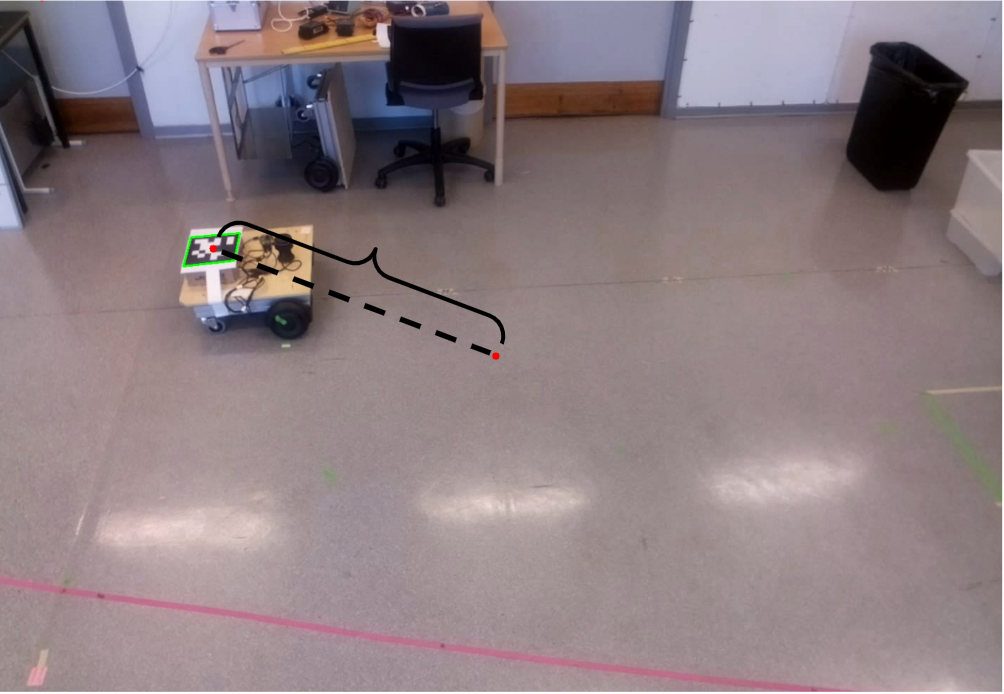
\includegraphics[scale=0.3]{images/resultcalc.png} 
   \caption{Example of a result from the detection algorithm. The green square outlines the result of the detected object and the red dot its' center. The error is the distance between the two dots as outlined by the black indicators.}
   \label{fig:resultcalc}
\end{figure}

\section{Auto-follow mode}
As a proof of concept, an auto-follow mode was developed which allowed the gimbal to follow the apriltag. This was made using the object detection algorithm from the result script coupled with a PI-controller which had the center of the image center as reference value. Due to time limitations this was not investigated any further.

\chapter{Experiments}
This chapter will describe the setup, procedure and evaluation of the two experiments that were performed.

\section{QoE Lab Experiment}
The goal of this experiment was to investigate the effects of latency on a camera operator, addressing goal \textbf{G1} of the thesis scope.

\subsection{Experiment Design}
The desire was to create a task that would be similar to what an operator would perform in a sea rescue scenario, while still making it easy to measure the performance of the operator. The the initial scenario using manual controls would be a drone, loitering around a point while also trying to focus the camera on it. 

As this required some type of movement inside the lab, the hoverboard was chosen to introduce movement in the test bed. With the video being the main feedback to the operator, pixel distance in an image was deemed to be a good metric for task performance. Furthermore, with the use of an apriltag, the amount of frames to be analyzed could be dramatically increased compared to manual analysis.

At first the desire was to have the gimbal box wirelessly sitting on top of the hoverboard, with the hoverboard moving in a circle in an upside-down loiter while the gimbal was looking up at a point in the ceiling, as shown in the leftmost picture in figure \ref{fig:testbed-ideas}. However, after some initial testing this was deemed to introduce several points of failure in the test bed:

\begin{itemize}
   \item Power had to be supplied via a powerbank.
   \item Network connection had to go over WiFi with substantially more delay and jitter than an ethernet cable-connection. 
   \item Using automatic detection, the lighting from the ceiling and windows reduced the contrast of the apriltag, making it harder to detect for the algorithm.
   \item When mounted, the gimbal box was higher than the lidar mounted on the hoverboard, confusing the location algorithm on the hoverboard.
\end{itemize}

In the end the loitering scenario was flipped, placing the gimbal box on top of a shelf looking down on the moving robot. The two test bed ideas can be seen in figure \ref{fig:testbed-ideas}. The hoverboard was started from a green marker in the room and ran two laps of a 2x1m elipse. It's path in the lab can be seen in figure \ref{fig:exp-setup}.

\begin{figure}[htp]
   \centering
   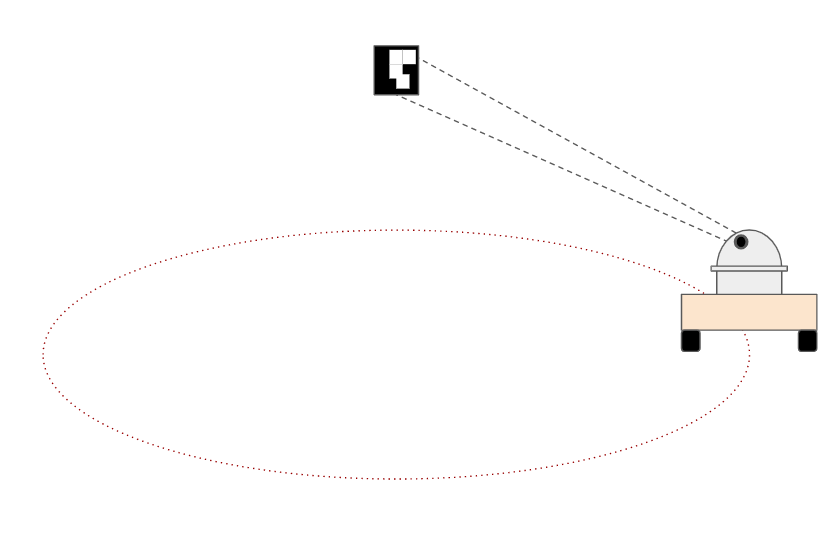
\includegraphics[width=.47\textwidth]{images/testbed1.png}\hfill
   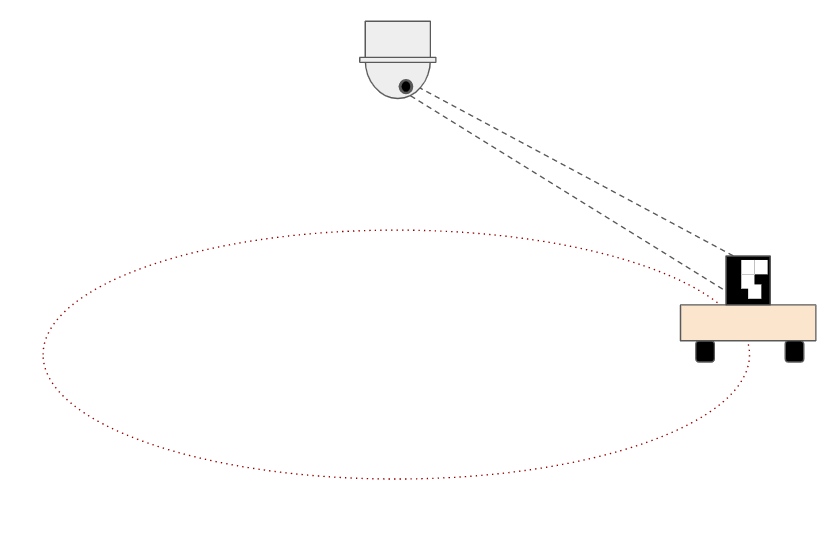
\includegraphics[width=.47\textwidth]{images/testbed2.png}
   \caption{To the left the initial idea of the experiment where the camera is looking up on the apriltag. To the right is the resulting scenario where the gimbal looks down on the apriltag placed on top of the hoverboard.}
   \label{fig:testbed-ideas}
\end{figure}

\subsection{Task}
The task for the operator was to keep the center of the screen, marked with a red dot as seen in \ref{fig:interface}, aligned with the center of the apriltag while it was moving in an elipse inside the lab.

\subsection{Experimental Setup}
The experiment was set up in a lab where the subject and the conductor sat at a desk with a high shelf behind them, obscuring the view towards the rest of the lab. Behind the shelf the robots used in the experiment were located. An illustration of the lab setup is provided in figure \ref{fig:exp-setup} and a photograph of the test bed is shown in figure \ref{fig:real-exp}.


\begin{figure}[!hbt]
   \centering
   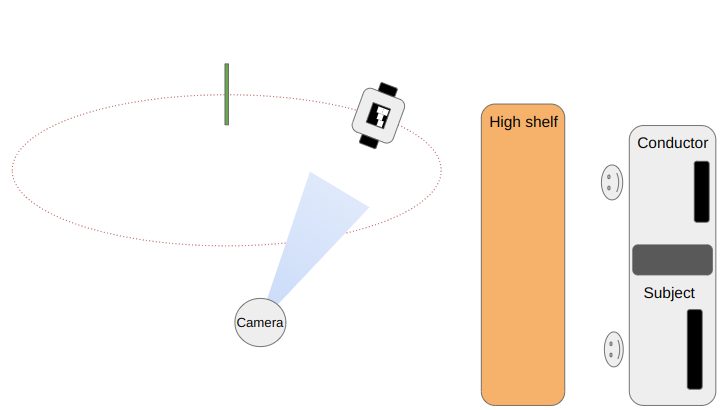
\includegraphics[scale=0.3]{images/exp-setup.png} 
   \caption{An overview of the experimental setup. To the right the experiment conductor and subject by a desk facing right. On the left side, behind the shelf, the test bed including the camera and the hoverboard are located. The camera is mounted at a height of 2.1 meters with the gimbal facing down.}
   \label{fig:exp-setup}
\end{figure}


\begin{figure}[!hbt]
   \centering
   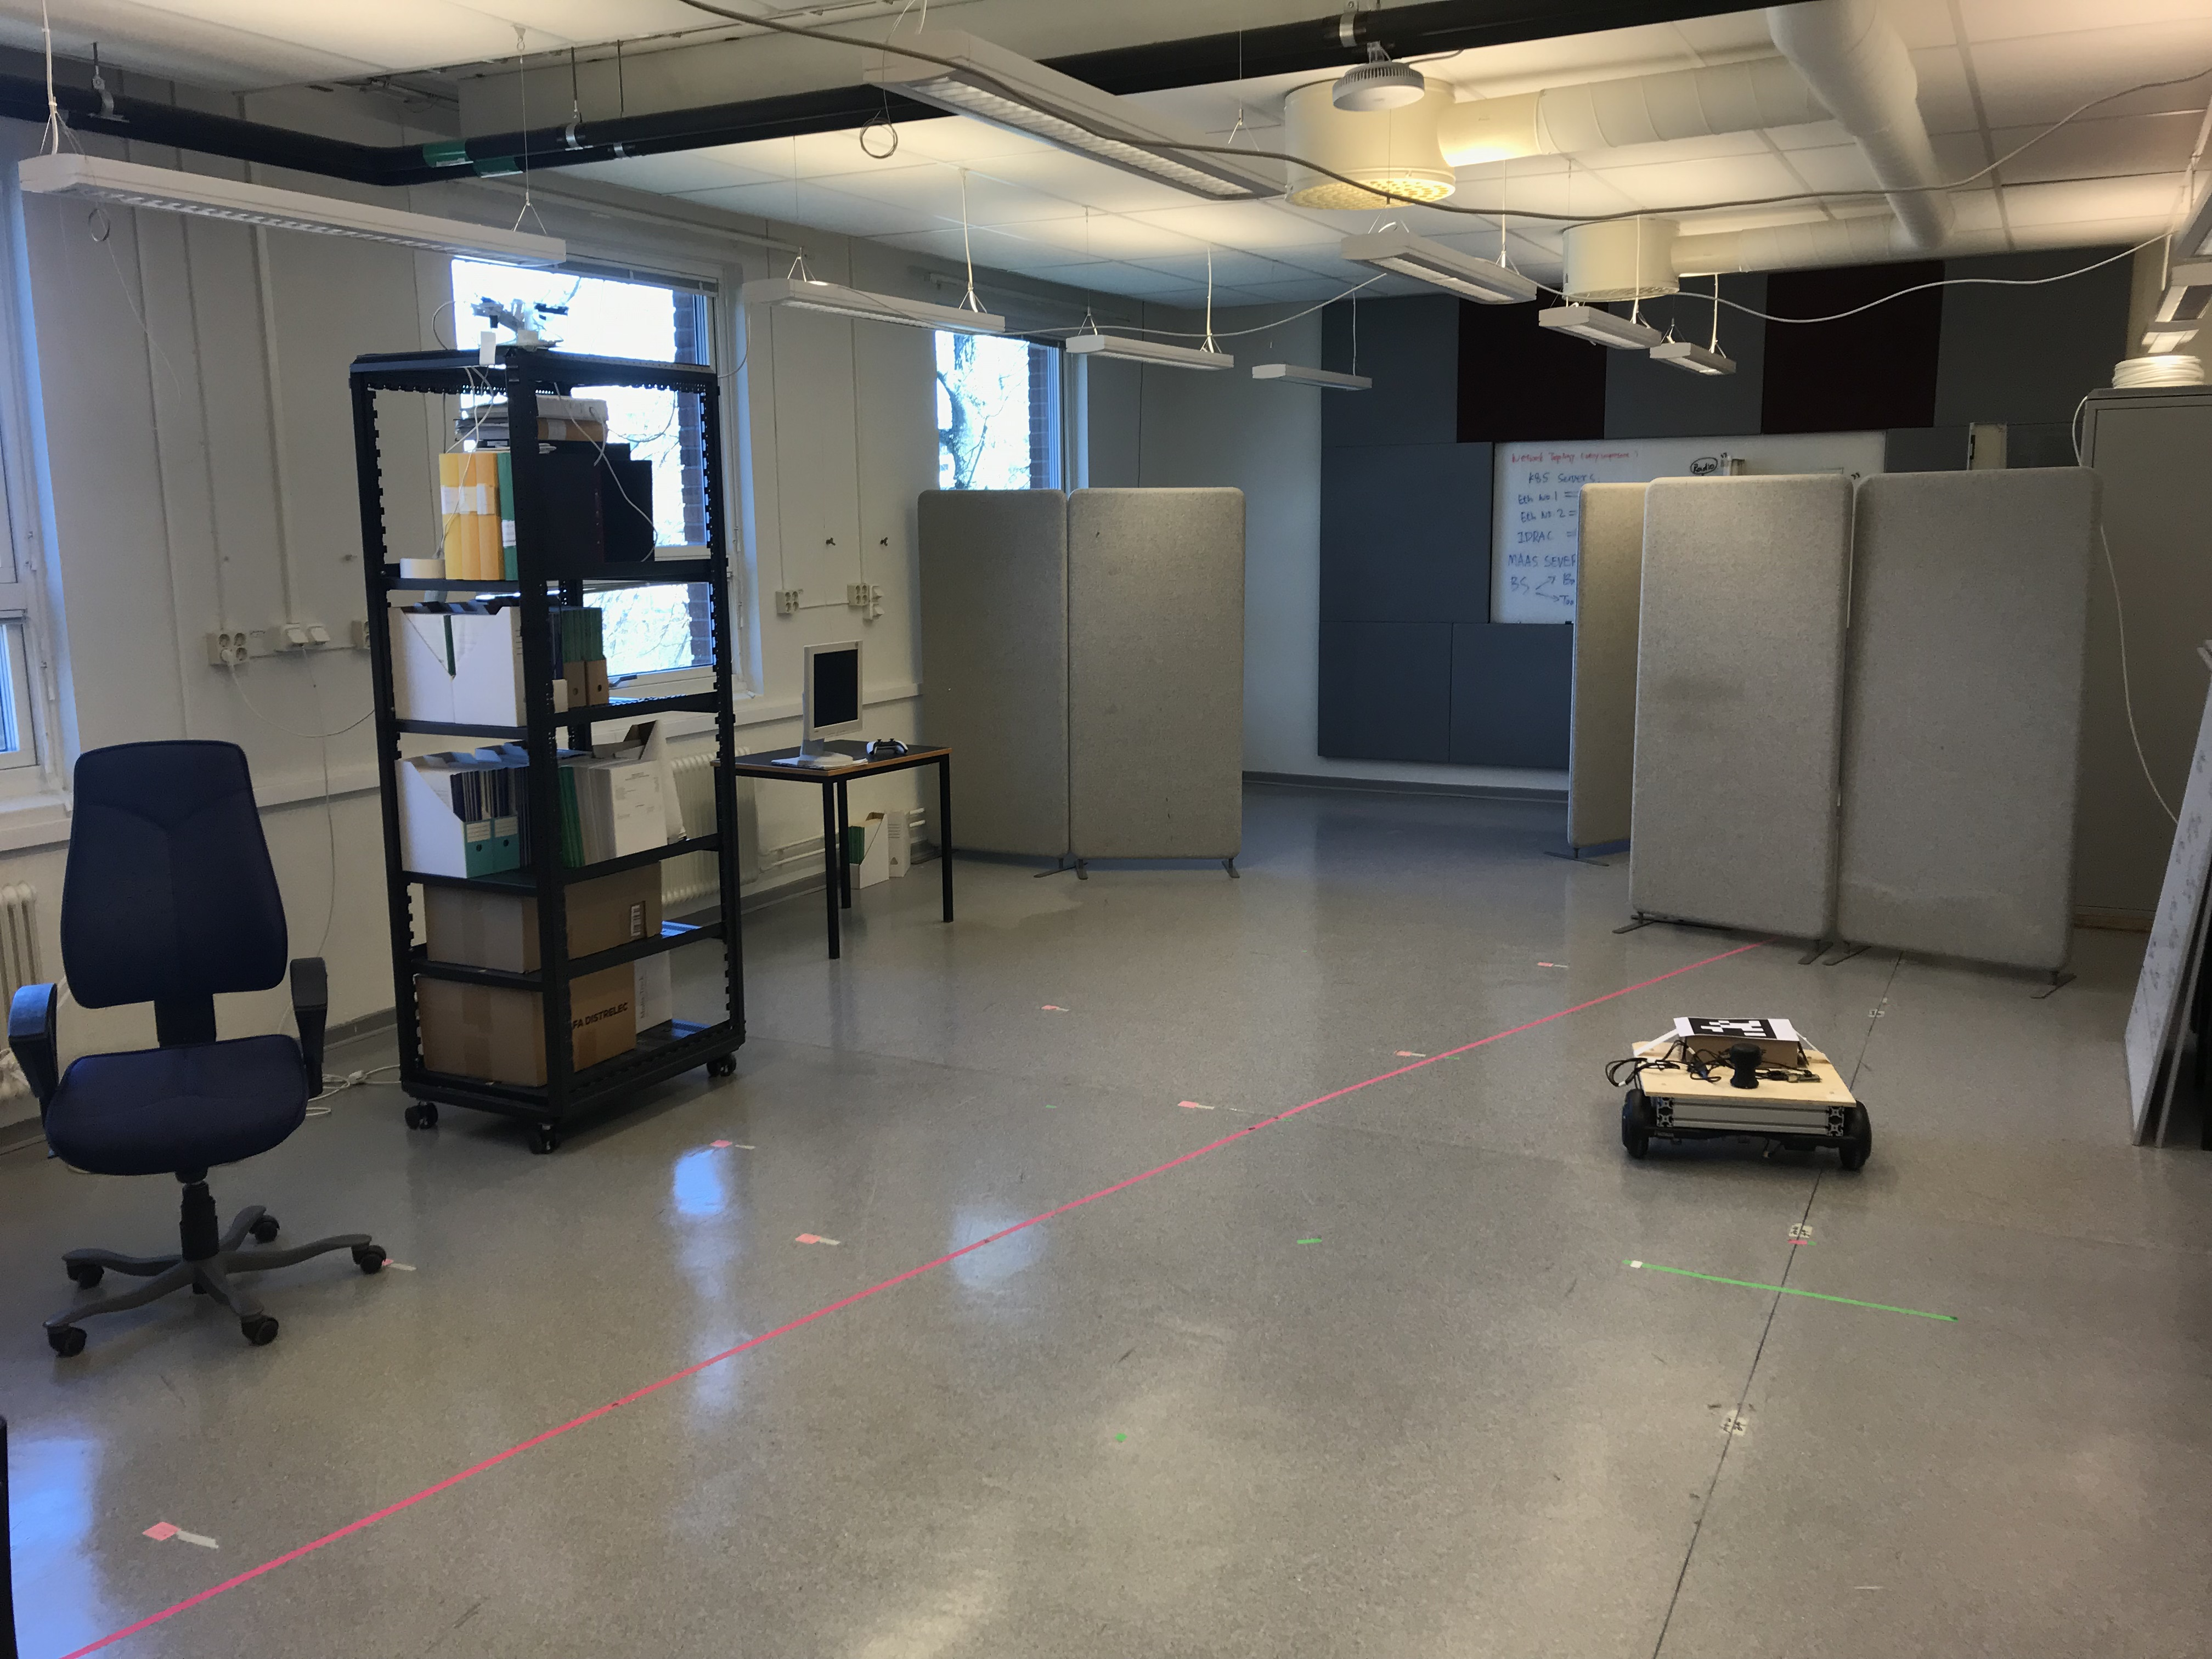
\includegraphics[scale=0.1]{images/testbed.jpg} 
   \caption{A picture of the test bed. On the left side there is a server rack with the drone box mounted on top. The hoverboard can be seen on the right side of the picture.}
   \label{fig:real-exp}
\end{figure}

\subsubsection{Test Subjects}
The subjects were recruited mostly from the conductor's network of contacts, as in order for the subjects to be covered by insurance during the experiment the subjects had to be either be students or employed by Lund University. Some of the participants came spontaneously while others booked a time in a spreadsheet provided by the conductor.

There was no compensation for the subjects other than home baked goods and a hot beverage, which were offered at the beginning of each experiment.

There were 10 test subjects, 4 women and 6 men, with an average age of 26.1 years where the youngest was 23 and the oldest 37. Furthermore, 5 of the subjects wore glasses and all were right-handed. 

They were also asked about their experience with games with first-person-view on the scale of 0 = "None", 1 = "Tried", 2 = ">10h", 3 = ">100h", 4 = ">500h", and the median result was 3.5 with 0 as the lowest and 4 as the highest. The subjects were also asked about their experience with flying drones using the same scale, and the median result was 0.5 with 0 as the lowest and 1 as the highest. 

\subsubsection{Lab Conditions}
The lab is located in the E-building at LTH, Lund University. It can also be mentioned that the windows in the room face north, so there was no risk of direct sunlight during the experiments.
The computer screen was 24' and the application was run on a machine with the following specifications:
\begin{description}
   \item[CPU] Intel Core i7-4770 @ 3.40GHz, 4 cores 8 threads
   \item[RAM] 16 GB
   \item[GPU] Mesa Intel HD Graphics 4600 (HSW GT2)
\end{description}

The gimbal box was connected to the gimbal control interface via ethernet cable.

\subsection{Experimental Procedure}
In this section each of the steps will be described in more detail. The experimental procedure is summarized in the table \ref{tab:task-timeline}.

\begin{table}[ht]
   \centering
   \caption{Task Timeline}
   \label{tab:task-timeline}
   \begin{tabular}{|c|l|l|}
   \hline
   \textbf{Time (approx.)} & \textbf{Task} & \textbf{Instruction} \\ \hline
   3 & Coffee and cookies & \\ \hline
   5 & Introduction & Tell the subject about what the study is about. \\
   & & Gather personal data + consent \\ \hline
   2 & SSQ & \\ \hline
   3 & Experiment walkthrough & What is going to happen \\
   & & Description of task \\
   & & Where to aim exactly on the apriltag \\ \hline
   2 & Warm-up & The subject gets to try the setup for one lap \\ \hline
   10 & Tests & 5 tests with added latencies [0, 200, 300, 400, 500] \\ 
   & & in random order \\ \hline
   2 & SSQ & \\ \hline
   3 & Interview & \\ \hline
   30 & Total & \\ \hline
   \end{tabular}
\end{table}

\subsubsection{Introduction}
The experiment starts with the subject being seated at the desk to read through the consent form. After this was signed the conductor clarified that the subject was free to ask any question during the experiment and could choose to interrupt it without declaring any reason. 

Then, the subject fill out the background information form where they also get to choose a four digit code which from that point is the only identifier of the subject and it's results. If the subject booked a time slot in the spreadsheet, they were at this point removed from it.

\subsubsection{Experiment Walkthrough}
The task was explained to the subject while a printed apriltag with a cross on it was shown, marking the spot where to aim on the tag. The particular apriltag printed for this experiment had two white and two black squares meeting in the middle, making the center easier to identify. The apriltag shown to the subject is shown in figure \ref{fig:apriltag}.

\begin{figure}[!hbt]
   \centering
   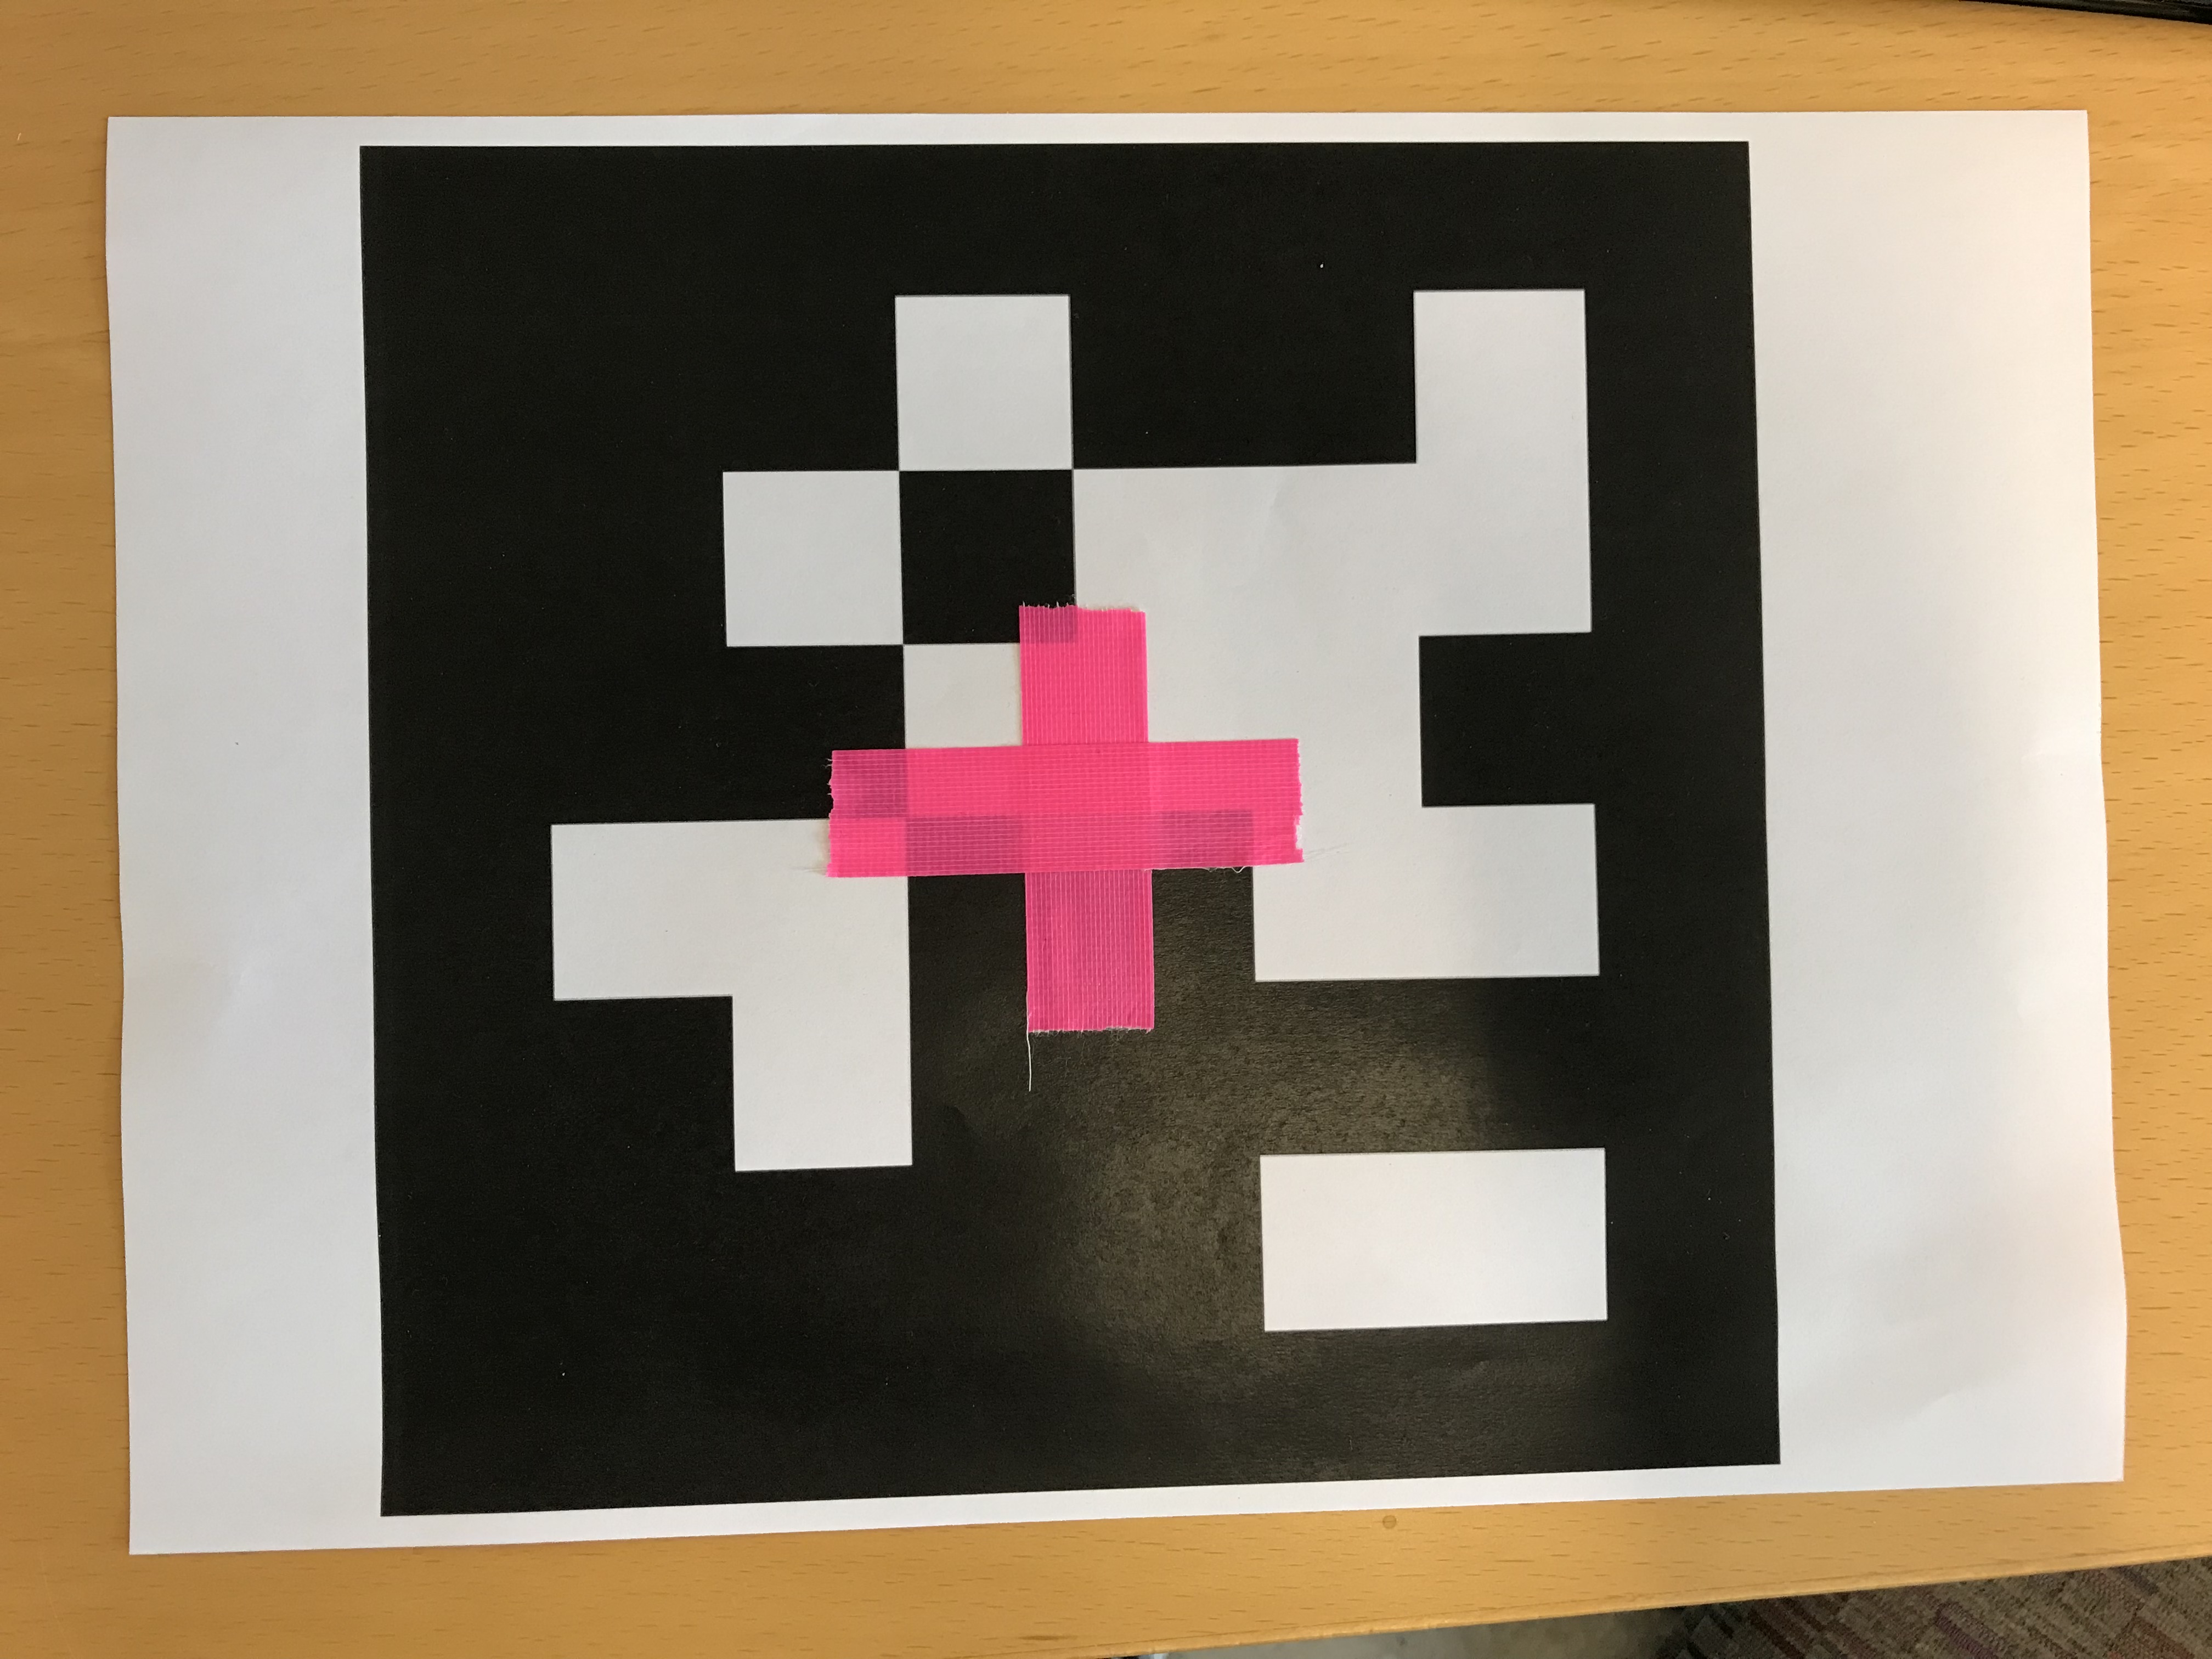
\includegraphics[scale=0.08]{images/apriltag.jpg} 
   \caption{The apriltag used to show the subject where to aim.}
   \label{fig:apriltag}
\end{figure}

The subject was then given a chance to try the system without any delay, and was given the controller and presented with the view, shown in figure \ref{fig:interface}. The hoverboard was started and ran for one lap in the same path that it would run during the test and the subject could try and follow it.

\begin{figure}[!hbt]
   \centering
   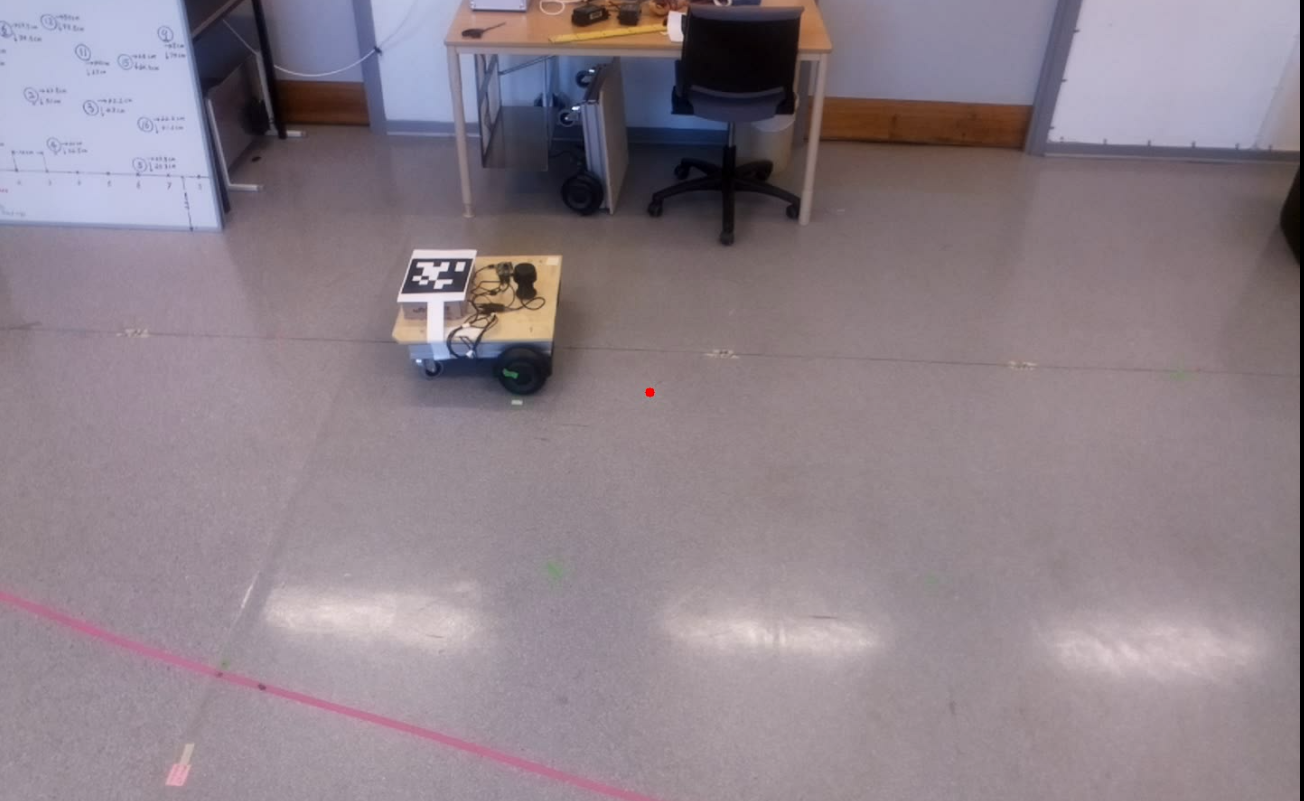
\includegraphics[scale=0.3]{images/interface.png} 
   \caption{The interface that the subject was presented with. The red dot in the middle of the screen is overlayed on top of the displayed video so that the subject has a better reference of the center of the screen.}
   \label{fig:interface}
\end{figure}

\subsubsection{Test Procedure}
After the task description and warm-up the tests commenced. The added latencies tested were 0, 200, 300, 400 and 600 and the order in which they were given to the subject was random. 
At the beginning of each trial the interface was restarted with one of the latencies induced in the system. The subject was then asked to put the red marker in the middle of the screen in the middle of the apriltag. When the subject confirmed that they were ready to start the conductor started the hoverboard. The subject followed the hoverboard for two laps, which took about 2 minutes in total.

After the laps were completed the interface was shut down and the subject was asked to rate the system by answering four different questions on a scale from 1 to 5. When the subject had answered the questions the next trial was started.

At the end of the fifth and last trial the subject got to fill in the sickness questionnaire was also asked a few interview questions by the conductor.

\subsection{Evaluation}
The following two sections will describe the quantative and qualitative methods that were used to evaluate the system.

\subsubsection{Quantative Evaluation}
To measure the performance of each subject, the result script described in section \ref{sec:resultscript} was used. This resulted in one CSV-file with about 2700 rows of data per trial. The start and end frames where extracted manually from the video of each trial and were saved in a separate file.  

\subsubsection{Qualitative Evaluation}
After each trial the subject answered a form with four questions about the system on a five degree scale, labeled 'Terrible' to 'Excellent'. The questions are shown in table \ref{tab:form-questions}. 

\setlength{\extrarowheight}{5pt}
\vspace{10pt}

\begin{table}[!hbt]
   \centering
   \begin{tabular}{|c|}
      \hline
      \textbf{How would you describe the controllability of the system?} \\
      \\
      Terrible \hspace{10pt} Poor \hspace{10pt} Fair \hspace{10pt} Good \hspace{10pt} Excellent \\    
      \\
      \hline
      \textbf{How would you rate your ability to perform the task?} \\
      \\
      Terrible \hspace{10pt} Poor \hspace{10pt} Fair \hspace{10pt} Good \hspace{10pt} Excellent \\    
      \\
      \hline
      \textbf{How pleasant was the system to use?} \\
      \\
      Terrible \hspace{10pt} Poor \hspace{10pt} Fair \hspace{10pt} Good \hspace{10pt} Excellent \\    
      \\
      \hline
      \textbf{How would you rate your impression of the system as a whole?} \\
      \\
      Terrible \hspace{10pt} Poor \hspace{10pt} Fair \hspace{10pt} Good \hspace{10pt} Excellent \\    
      \\
      \hline
   \end{tabular}
   \caption{The questions asked for each delay after each trial.}
   \label{tab:form-questions}
\end{table}

\vspace{10pt}

Right after the last trial the subject filled out the SSQ once more. Then, a brief interview was conducted with questions about the system and experience in general. The questions can be seen in table \ref{tab:interview-questions}.

\setlength{\extrarowheight}{5pt}
\vspace{10pt}

\begin{table}[!hbt]
   \centering
      \begin{tabular}{|c|}
         \hline
         \textbf{1. What was your general experience of controlling the camera?} \\
         \hline
         \textbf{2. Did you experience any difference in the controls between the trials?} \\
         \hline
         \textbf{3. Was there any part of the track that was harder than any other?} \\
         \hline
         \textbf{4. Do you think the system would have been usable with the worst experimental conditions?} \\
         \hline
         \textbf{5. Do you think training would have helped an operator get better using the system?} \\
         \hline
      \end{tabular}
   \caption{The interview questions asked by the conductor after the last trial.}
   \label{tab:interview-questions}
\end{table}

\vspace{10pt}

\subsection{Known Sources of Error}

\subsubsection{Ecological validity}
The future operators of the system are to be the volunteers of SSRS, which have a wide variety in age and background. Thus,there are three main concerns with the ecological validity of the study. Firstly, the subjects were all either students or researchers at Lund University. Secondly, the average age of the subjects was low. Lastly, the sample size was only ten people. 


The first and second concerns are difficult to compensate for, as only employees or students at the university could be used as subjects due to the university insurance. There are of course people of different ages and backgrounds working and studying at the university, but due to time restraints as well as lack of compensation for the subjects, most came from the conductor's network of contacts.

The last concern is mainly an issue with the qualitative results, as the amount of quantitative data could be increased by having each subject do several laps. Each subject generated around 13 500 data points in all five trials, resulting in about 135 000 data points for pixel error over all subjects.

\subsubsection{Frame detection accuracy}
The detection algorithm used to calculate the distance from the center of the apriltag to the center of the screen could sometimes during fast camera movements not detect the apriltag. This resulted in a NaN value at that particular frame. The average percentage of frames detected where 85\%, with a minimum of 80\% and a maximum of 89\%.

To easen analysis, all NaN values, i.e frames where no apriltag was detected in the frame, were linearly interpolated. To illustrate this one result is shown before and after interpolation in \ref{fig:raw-vs-interpolated}. 

\begin{figure}[!hbt]
   \centering
   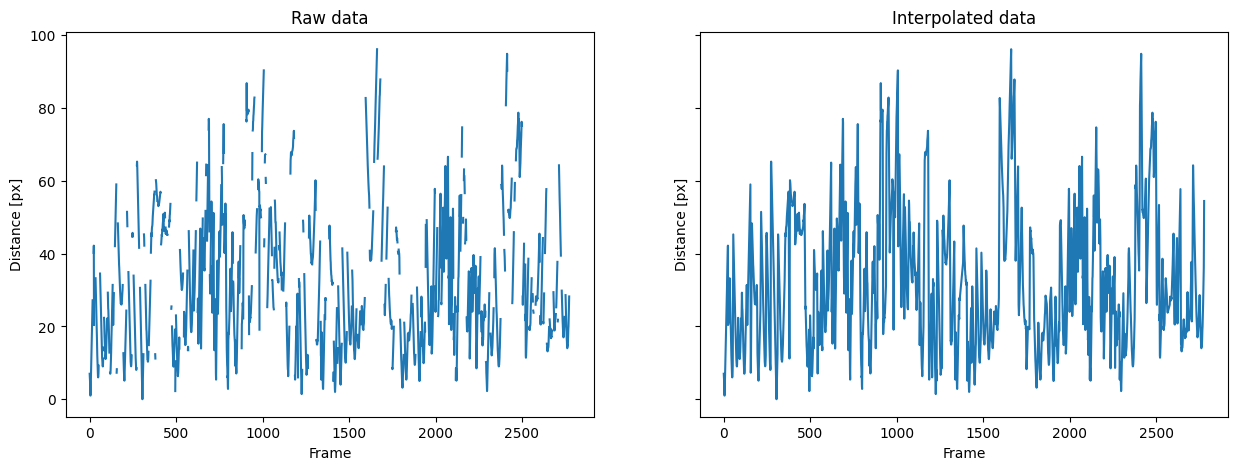
\includegraphics[scale=0.5]{images/raw-vs-interpolated.png} 
   \caption{Results for one trial: to the left the result with NaN-values and to the right interpolated result.}
   \label{fig:raw-vs-interpolated}
\end{figure}

\subsubsection{Difficulty of the task}
The center of the apriltag did not have a very clear center, which could have made it difficult for the subject to complete the task. To remedy this, a printed apriltag where the center was marked out was given to the subject. However, the subject could still have had difficulty identifying the exact center of the apriltag during the trial.

\subsubsection{Control Choppiness}
\label{sec:control-choppiness}
The control of the gimbal is done through a command sent to the drone with two angles for pitch and yaw. The drone then moves the gimbal to the desired angles. Although the angle was provided as a float, small increases from the joystick did not produce movement in the gimbal. This resulted in the control being choppy in relation to the continous input of the joystick. The choppiness also increased when looking at more distant points. 

\section{Field testing}
The goal of this experiment was to integrate the software built for the test bed into the existing drone system, addressing goals \textbf{G3} and \textbf{G4} of the thesis scope. 

\subsection{Preparations}
For the experiment the gimbal control interface was modified to run with the software configured on the actual drone. The video and recording component was entirely removed and the IP address which the program connected to was changed to that of the 4G modem on the drone.

In order to compare the new controls to the already existing ROI-mode, a button on the controller was mapped to switch between joystick-mode and ROI-mode, which when activated uploaded a pre-programmed GPS-point for the drone to look at.

\subsection{Outdoor Conditions}
The weather was sunny with almost no clouds. The ground level wind was estimated to be around 5-9 m/s and the temperature was around 12 degrees Celsius.

\subsection{Procedure}
A flight plan of 17 waypoints including a loiter-waypoint was uploaded to the drone. The flight plan can be seen in \ref{fig:flight-plan}. The first and the last waypoints were close to the launch and the rest were placed on a route out in the archipelago. The drone was launched in manual mode and was circled around the operators to confirm that all the systems were working. The gimbal control software was also confirmed to be working during this phase, and the latency of the control was estimated to be between one and two seconds. The drone was then switched into auto mode and the flight plan was started.

The SSRS have a permit to fly BVLOS in the Gothenburg archipelago. Contact was kept with the control tower before and during the entire flight.

\begin{figure}[!hbt]
   \centering
   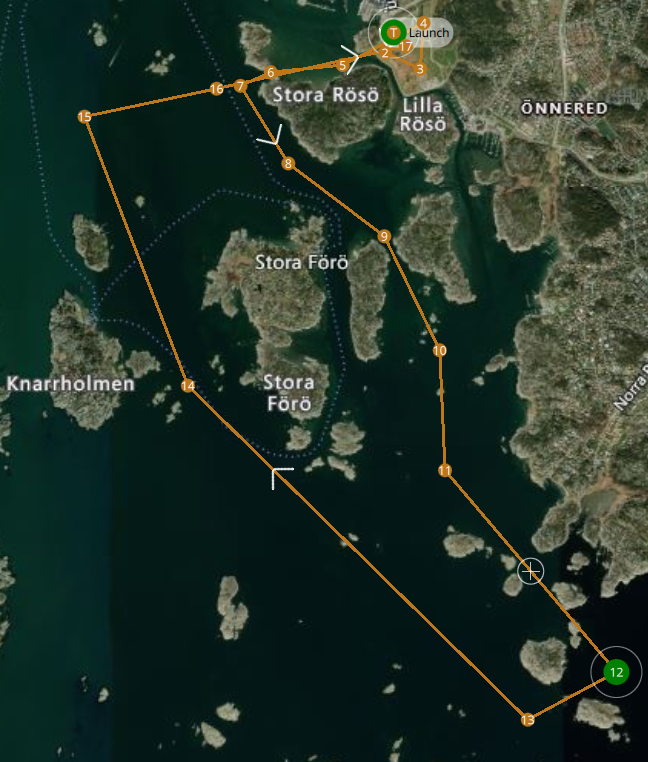
\includegraphics[scale=0.4]{images/flight-plan.png} 
   \caption{The waypoints of the flight plan. The 12th waypoint was a loiter waypoint.}
   \label{fig:flight-plan}
\end{figure}

\chapter{Results}
This chapter will go through the main findings of the experiments. The quantative measurements will first be presented followed by the results from the forms and interviews. Lastly, the results from the field testing will be presented.

\section{QoE Experiment}
In this section the quantative and qualitative results of the QoE experiment are presented and discussed.  

\subsection{Quantative measurements}
In \ref{tab:averages} the mean and standard deviation of the different delays are presented. The values are also visualized in plot \ref{fig:avg-std}. A clear trend can be seen where both the mean and standard deviation increase with the delay. An interesting feature of the data is that the mean after 400ms starts to increase at a non-linear rate, while the standard deviation has a more or less linear increase all throughout the added delays.

\begin{table}[ht]
   \centering
   \begin{tabular}{|c|c|c|}
   \hline
   \textbf{Delay} & \textbf{ Mean} & \textbf{Std. deviation} \\
   \hline
   0 & 29.804138 & 18.030196 \\ \hline
   200 & 35.234192 & 22.347311 \\ \hline
   300 & 41.538190 & 26.805780 \\ \hline
   400 & 46.048449 & 28.718249 \\ \hline
   600 & 61.811312 & 37.226394 \\ \hline
   \end{tabular}
   \caption{Table caption goes here.}
   \label{tab:averages}
\end{table}


\begin{figure}[!hbt]
   \centering
   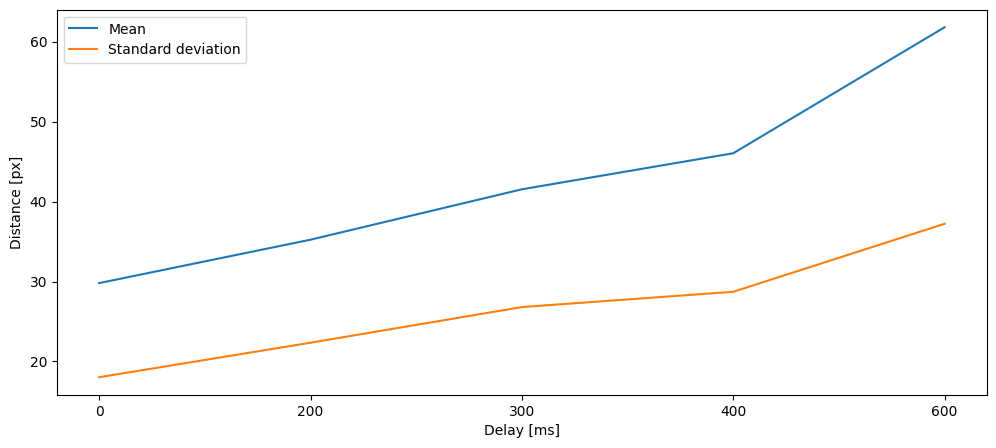
\includegraphics[scale=0.5]{images/avg-std.png} 
   \caption{Pixel error average and standard deviation for all delays. Delays 100 and 500 are added on the x-axis for correct scale.}
   \label{fig:avg-std}
\end{figure}

In figure \ref{fig:ecdf} the empirical cumulative distribution functions (ECDF) for the results of each delay are shown. The x-axis represents the value which the entry has while the y-axis represents the percentage of entries that are less than or equal to the x-axis value. The increase in both average and mean can be clearly observed as the delay increases. It can also be deduced that the distance between the center of the ECDF distributions for 0ms and 200ms is much smaller than that between the curves for 400ms and 600ms. This could indicate that the added 200ms added delay had a larger impact at 400ms than at 0 ms.

\begin{figure}[!hbt]
   \centering
   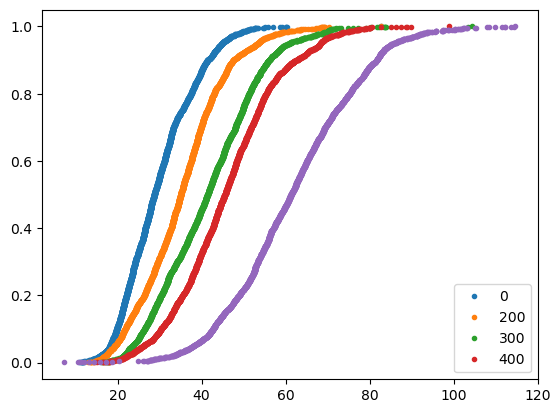
\includegraphics[scale=0.5]{images/ecdf.png} 
   \caption{ECDF of the total pixel error averaged over all subjects. The curves show the distribution of the error for each delay. A larger inclination suggests a larger spread and the more to the right the curve is, the larger the average error.}
   \label{fig:ecdf}
\end{figure}

In figure \ref{fig:hoverboard-pos} all the values from the trials have been averaged and the position of the hoverboard has been superimposed. In this plot one can see that the final corner of the track is the most difficult, and that the very end and early beginning of the track are the easiest. 

\begin{figure}[!hbt]
   \centering
   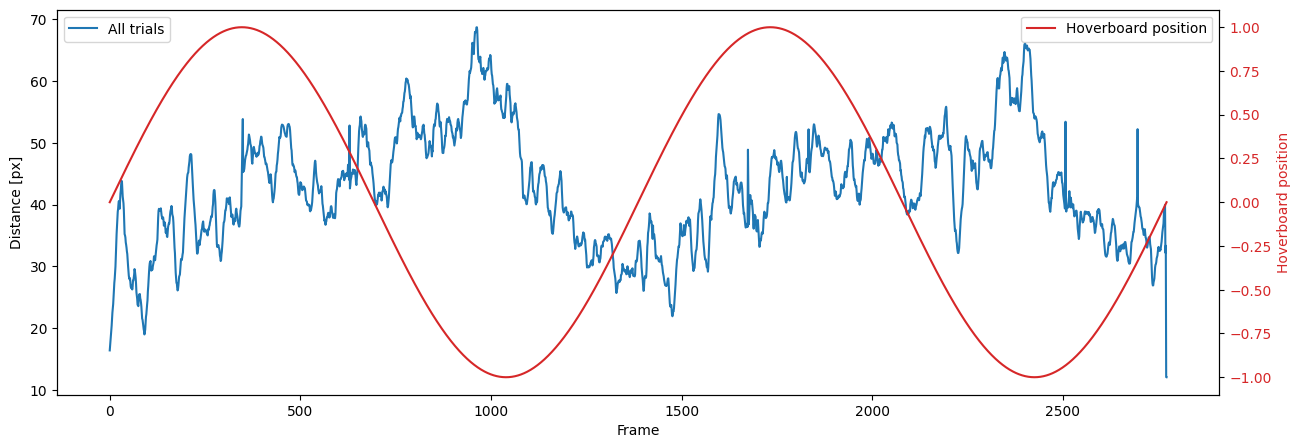
\includegraphics[scale=0.4]{images/hoverboard-pos.png} 
   \caption{All trials averaged with hoverboard position superimposed. The error steadily increases up until the end of the last corner where it decreases rapidly.}
   \label{fig:hoverboard-pos}
\end{figure}

To see the performance over the course of the hoverboard's track for each delay, the trials of all subjects were summarized on a particular delay alongside the position of the hoverboard. This is shown in \ref{fig:0vs600}, where all trials with 0ms and 600ms added delay are averaged on each frame. The more transparent blue and green lines represent the average over all trials while the darker lines are a rolling average of the data. The red line represent the position of the hoverboard.
It can be seen that there is a    

\begin{figure}[!hbt]
   \centering
   \makebox[\textwidth]{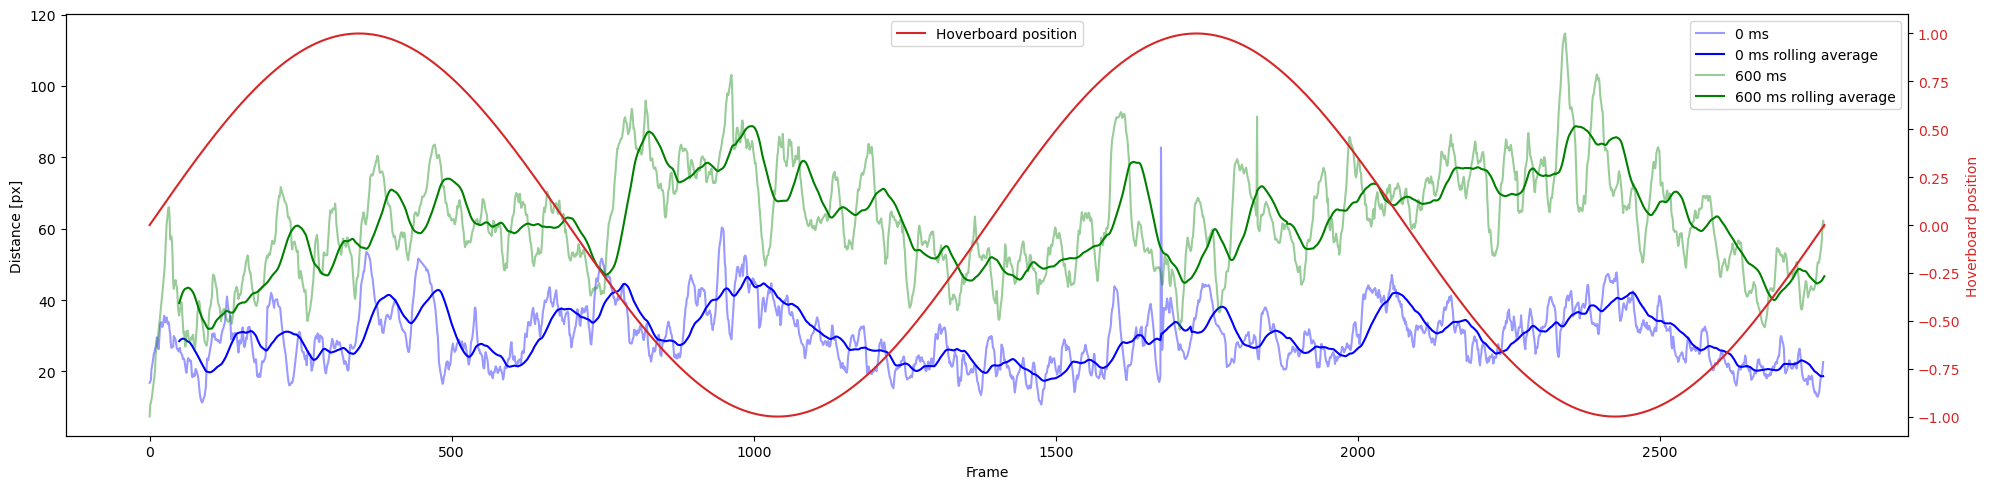
\includegraphics[scale=0.35]{images/0vs600.png}}
   \caption{Total trials for latencies 0 and 600 averaged over all subjects.}
   \label{fig:0vs600}
\end{figure}


\subsection{Forms and interviews}
In this section the results from the forms and interviews are presented and discussed.

\subsubsection{Trial forms}
In \ref{fig:form-ans} the answers from the questionnaires filled out after each trial are averaged over all subjects and visualized as a grouped bar chart. It is important to note that the jumps in delay are not uniform. The questions can be seen in \ref{tab:form-questions}. 

Here follows a brief analysis of the results for each question in \ref{fig:form-ans}
\begin{description}
   \item[1: Controllability] 
   The controllability decreases dramatically over all delays. Although the ratings decrease with added delay, the answers suggest that the sence of controllability did not differ much between 400ms and 600ms added delay, and that the answers could plateau with further added delay.  

   \item[2: Ability to perform task] 
   The average ratings for 200ms, 300ms, and 400ms are very similar. The added delay seems to have had little effect on the impression of their task performance, in spite of the quantative results showing a significant difference in pixel error. The subject's answer does however depend heavily the subject's interpretation of the task and how close is "good enough".
 
   \item[3: How pleasant was the system to use]
   The ratings of the pleasantness of the system seem to decrease steadily with added delay for each interval.

   \item[4: Impression of the system as a whole] 
   The system with 0ms added delay clearly made a better impression on the subjects. An interesting feature of the answers is that the systems with 200ms and 300ms have gotten the exact same rating.

\end{description}

\begin{figure}[!hbt]
   \centering
   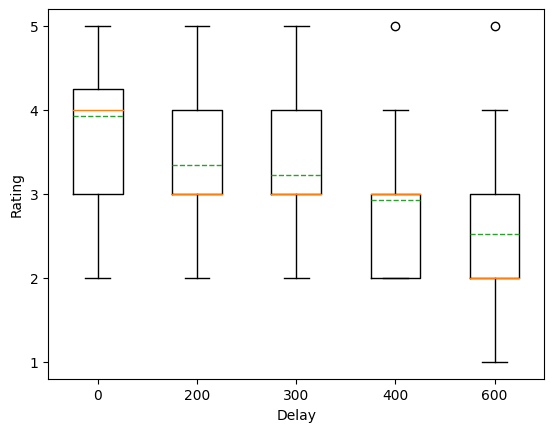
\includegraphics[scale=0.6]{images/form-ans.png} 
   \caption{Form answers averaged for all subjects for each delay.}
   \label{fig:form-ans}
\end{figure}

\subsubsection{Simulator Sickness Questionnaire}
In \ref{fig:ssq-ans} the difference in SSQ answers before and after the trials been averaged over all subjects. The largest response increase is on symptom four, namely "eye strain", which had an average increase of  0.5 with four out of all the subjects reporting an increase. The next two highest symptoms were "fullness of head" and "blurred vision". 

The results from the SSQ suggest a small increase in  symptoms after the trials, but the increase is not large enough to be considered significant for a sample size of only 10 subjects.

\begin{figure}[!hbt]
   \centering
   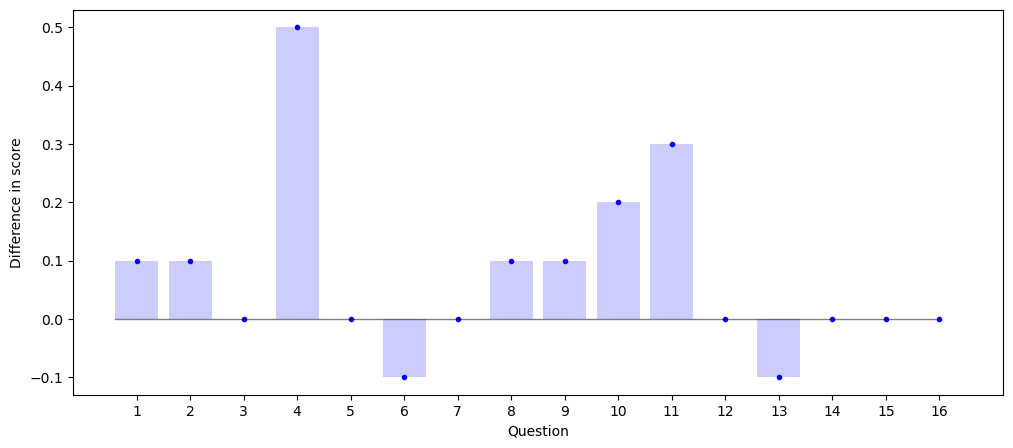
\includegraphics[scale=0.6]{images/ssq-results.png} 
   \caption{Difference in SSQ answers from before and after the trials on a scale from 0 to 4.}
   \label{fig:ssq-ans}
\end{figure}

\subsubsection{Interviews}
The answers to the interview questions will be summarized in this section.

\titleformat{\paragraph}[hang]{\normalfont\small\bfseries}{\theparagraph}{1em}{}
\titlespacing*{\paragraph}{0pt}{3.25ex plus 1ex minus .2ex}{1em}

\paragraph{1. What was your general experience of controlling the camera?}
A majority of the subjects reported that camera controls felt choppy, which is probably caused by the controls, explained in section \ref{sec:control-choppiness} on control choppiness. The subjects also reported that the controls felt very different throughout the trials. Some subjects also said that they grew more accustomed to the controls as the trials progressed.

Some quotes from the subjects are presented below.
\begin{description}
   \item[Subject 4545] "Had this been my day job I would have jumped out the window". 
   \item[Subject 1111] "Intuitive, sometimes there was delay that made it diffficult."
\end{description}

\paragraph{2. Did you experience any difference in the controls between the trials?}
All the subjects felt reported a difference in the trials. Usually subjects had a clear view on which trials were the easiest or the most difficult.

\paragraph{3. Was there any part of the track that was harder than any other?}
Almost all subjects reported that the last corner was the most difficult out of the entire track. This is supported by the quantative results as a visible spike in pixel error is present at that point in the track throughout all trials.
Some also stated that it was easier when the hoverboard was closer to the camera. This could be due to the effect of camera's choppiness which was less noticable short range, as explained in section \ref{sec:control-choppiness}.

\paragraph{4. Do you think the system would have been usable with the worst experimental conditions?}
On this question the answer of the subjects varied. A couple gave an absolute no, while others said that it depended on how exact one had to follow the object. 

\paragraph{5. Do you think training would have helped an operator get better using the system?}
All the subjects responded that training would improve one's performance in the system and that they got better at the task as the trials progressed. 

\section{Field Testing}
The gimbal control software integrated successfully into the running system and did not interfere with the controls during the course of the experiment. Thus, the goal \textbf{G3} was reached successfully.

The two different modes of operation were tested and the results are presented in the following sections.

\subsection{Manual Control}
During the initial loiter, the plane's orientation changed quickly depending on where the plane was facing with respect to the direction of the wind. This made the gimbal very difficult to control manually, with the delay of the controls making it almost impossible to manually compensate with the joystick when the plane made an aggressive roll or yaw.

After the plane had left the initial loiters it had more time flying straight. During this time the camera was much easier to control manually, as the plane was more stable and the orientation was remained the same for an extended amount of time. 
Between waypoint 11 and 12, a boat was spotted slightly beside the plane. The gimbal operator decided to try and follow the boat. Although the delay made it more difficult to control the gimbal than in the lab experiment, the boat was successfully followed for a short time. An illustration of the event can be seen in \ref{fig:boat-follow}. It was also observed that the operator could predict the position of the boat, allowing preemptive gimbal movements to compensate for the delay. 

\begin{figure}[htp]
   \centering
   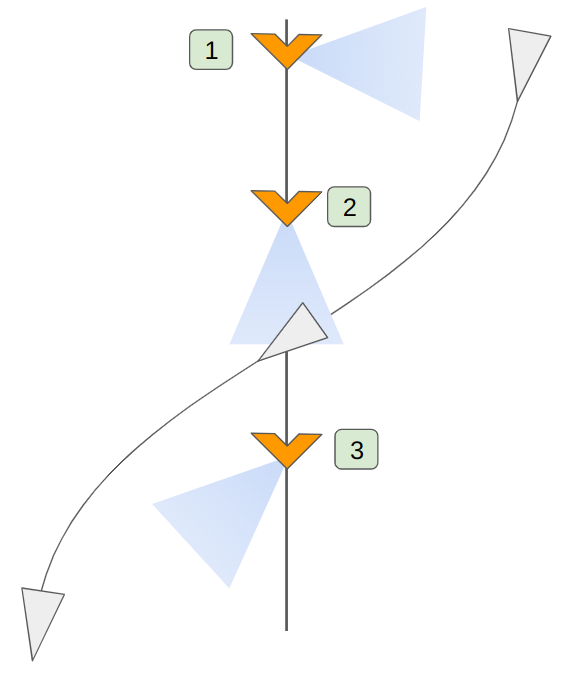
\includegraphics[width=.33\textwidth]{images/drone-boat-illustration.png}
   \caption{Illustration of the drone following the boat. The orange shape is the drone and the triangle the boat. The green boxes indicate points in time and the blue cone the drones field of view which was changed by the gimbal control software during flight.}
   \label{fig:boat-follow}
\end{figure}

Another observation from the experiment is that, being a fixed wing aircraft, the operator's ability to control the camera relies heavily on the manouvering of the aircraft, which means that improving the controls of the actual aircraft would improve the experience of controlling the camera significantly. 

\subsection{ROI Control}
The ROI-mode was activated on waypoint 12, and worked well when the perspective of the drone was changing rapidly. However, there were some inconsistencies in the altitude data for the points which caused the camera to point at a point below the surface of the earth. The point was adjusted by raising the altitude provided to the GPS-point. 

It could also be observed that increasing the loiter-radius gave a better image as the inexactness of the GPS-point was less impactful.


\chapter{Discussion}

\section{Comparison with State-of-the-Art}

\section{Impact}

\section{Limitations}

\section{Weaknesses}

\section{Strengths}

\section{Benefits, Ethics and Sustainability}


\chapter{Conclusion}
In this chapter the goals presented in section \ref{sec:scope} will be evaluated.

\begin{description}
   \item[G1]  A test bed running one the hardware provided by the SSRS was implemented successfully.

   \item[G2]  In the quantative results from the experiment, a clear trend can be seen that additional delay has a negative effect on the subject's ability to control the camera. Furthermore, the same increase in delay seem to have a larger effect on the subject's performance when introduced at a higher delay.  

   When taking into account the subject's rating of the system, it can be seen that the experience of a user is not always proportional to the worsening of QoS parameters. A slight increase in simulator sickness was observed, although it was not statistically insignificant with only 10 subjects.

   \item[G3] The results from the field testing shows that the gimbal software could be integrated with the system running on the real drone.

   \item[G4] The manual controls were deemed suitable when the plane was flying in straight lines and when surveying or following a moving. When loitering the already existing ROI-mode was found to be more suitable.
\end{description}

\chapter{Future Work}
The test bed developed in the thesis work could be used for more experiments in a lab environment. It would be interesting to look at the effect of other delays as well as the effects of other network parameters such as jitter or image quality. In the future it would also be interesting to perform studies on when the drone is either moving or in flight.
The modified test bed will(/can?) also be used by the SSRS as starting point for controlling the camera on the drone, and will help to evaluate the use case of drones for sea rescue further.

% Should use consistent formatting when it comes to Names ("FirstName LastName", or "F. LastName")
%\printbibliography
\makebibliography{MyMSc}

\end{document}